\documentclass[10pt,twocolumn]{article}
\usepackage{graphicx}
\usepackage{amsmath}
\usepackage{float}
\usepackage{hyperref}
\usepackage{geometry}

% Réglages compacts
\geometry{margin=1.6cm, columnsep=1.1cm}
\setlength{\parskip}{0pt}
\setlength{\parindent}{1em}

\title{Analyse temporelle, structurelle et communautaire \\
du réseau hospitalier de contacts}
\author{Projet Graph Mining}
\date{\today}

\begin{document}
\maketitle

\newpage

% ============================================================
\section{Introduction}
% ============================================================

Les réseaux de contacts hospitaliers constituent une source d'information essentielle pour comprendre la dynamique d'interactions entre personnel médical, administratif et patients. Leur étude permet d'interpréter :

\begin{itemize}
    \item les mécanismes d'organisation sociale au sein d'un établissement de santé ;
    \item la propagation potentielle d'informations ou d'agents pathogènes ;
    \item la centralité de certains rôles et leur implication dans la structure du réseau.
\end{itemize}

L'objectif est d'obtenir une compréhension précise de la structure du réseau et du rôle joué par chaque catégorie d'acteurs.

% ============================================================
\section{Mesures de centralité}
% ============================================================

Afin de caractériser la structure du réseau hospitalier, nous avons calculé plusieurs mesures de centralité : \textit{degree}, \textit{strength}, \textit{betweenness}, \textit{closeness}, \textit{eigenvector centrality} et \textit{PageRank}. 
Ces mesures permettent d'identifier quels individus occupent des positions importantes dans le réseau et jouent potentiellement un rôle clé dans la transmission de pathogènes.

\subsection{Degree centrality}

Le \textit{degree} correspond au nombre d'individus distincts avec lesquels un nœud a interagi.
Cette mesure met en évidence les \textit{hubs}.
Dans notre réseau, ce sont principalement les infirmiers (NUR), suivis par certains médecins (MED), ce qui est cohérent avec leurs rôles professionnels.

\subsection{Strength}

Le \textit{strength} correspond à la somme des poids des arêtes incidentes, c'est-à-dire la durée cumulée des contacts.
Cette mesure permet d'identifier les \textit{super-contacteurs}.
Nos résultats confirment que les NUR sont de loin les principaux super-contacteurs.

\subsection{Betweenness centrality}

La \textit{betweenness} mesure la proportion des plus courts chemins passant par un individu.
Les nœuds ayant une betweenness élevée jouent un rôle de pont entre différentes parties du réseau.
Certains infirmiers et médecins occupent ce rôle, ce qui indique qu'ils relient plusieurs groupes structuraux (patients, autres personnels).

\subsection{Closeness centrality}

La \textit{closeness} calcule à quelle distance moyenne un individu se trouve de tous les autres.
Une valeur élevée indique une capacité à atteindre rapidement l'ensemble du réseau.
Les NUR présentent également des valeurs élevées, en raison de leur position dans le cœur du réseau.

\subsection{Eigenvector centrality}

L'\textit{eigenvector centrality} reflète l'influence globale d'un individu : un nœud est considéré comme important s'il est connecté à d'autres nœuds importants.
Les NUR et certains MED dominent également cette mesure, confirmant leur rôle central.

\subsection{PageRank}

Le \textit{PageRank}, pondéré par la durée des contacts, fournit une mesure similaire à l'eigenvector centrality mais plus sensible aux longues interactions.
Les super-contacteurs identifiés via le \textit{strength} sont également en tête du PageRank.

\subsection{Hubs et super-contacteurs}

L'analyse des centralités révèle que :
\begin{itemize}
    \item les NUR et MED occupent les positions les plus centrales selon toutes les mesures ;
    \item ils sont à la fois top-degree, top-strength, mais aussi élevés en betweenness, eigenvector et PageRank ;
    \item les PAT et ADM sont en revanche en périphérie du réseau.
\end{itemize}

Ces résultats sont parfaitement cohérents avec l'étude originale, dans laquelle six HCWs (infirmiers + médecins) représentent 42\% de l'ensemble des contacts avec les patients, confirmant la présence de super-contacteurs.

Ainsi, notre analyse étend celle de l'article : alors que les auteurs identifiaient les super-contacteurs via le nombre et la durée des contacts, nous montrons que ces mêmes individus sont également centraux selon plusieurs mesures avancées, ce qui renforce l'idée qu'ils peuvent agir comme des \textit{super-spreaders} potentiels.

% ============================================================
\section{Graphes modèles (Model Graphs)}
% ============================================================

Dans cette section, nous comparons le réseau hospitalier réel à deux graphes modèles classiques vus au cours : le modèle d'Erdős–Rényi (ER) et le Configuration Model (CM). 
Ces modèles servent de \textit{null models} permettant d'évaluer si les propriétés du réseau réel peuvent être expliquées par des mécanismes simples tels que l'aléa pur (ER) ou la distribution des degrés (CM), ou s'il présente une structure sociale non aléatoire.

\subsection{Comparaison avec le modèle d'Erdős–Rényi}

Le modèle ER $G(N,q)$ génère un graphe aléatoire avec le même nombre de nœuds $N$ que le réseau réel et avec une probabilité $q$ d'existence d'une arête telle que le degré moyen corresponde à celui du réseau hospitalier.
La comparaison des distributions de degrés montre que le réseau réel est beaucoup plus hétérogène que le modèle ER : les degrés varient de 6 à 61 dans le réseau réel, alors qu'ils se situent entre 18 et 41 dans le graphe ER.

En échelle logarithmique, la distribution réelle présente une queue plus lourde et révèle la présence de \textit{hubs} (notamment des infirmiers), tandis que le graphe ER montre une distribution beaucoup plus concentrée autour de son degré moyen, caractéristique d'une loi de Poisson. 
Cela confirme que la structure du réseau hospitalier ne peut pas être reproduite par un graphe aléatoire simple.

\begin{figure}[H]
\centering
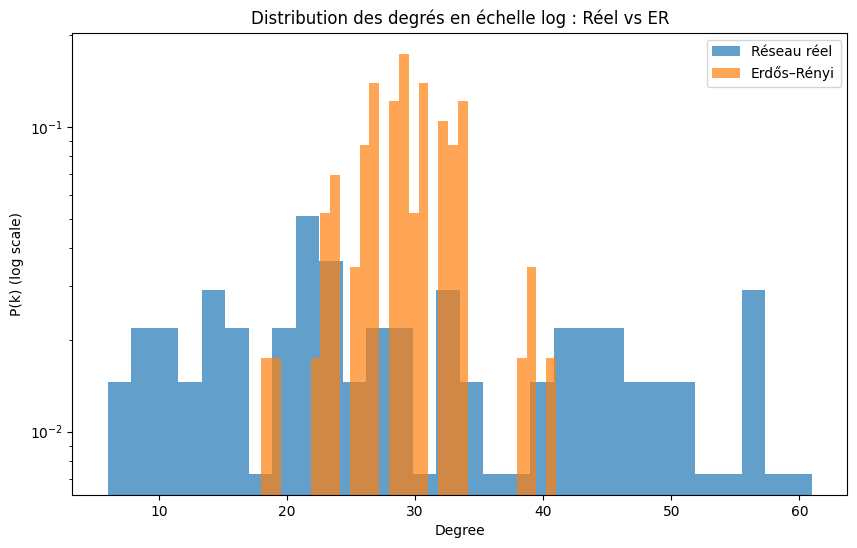
\includegraphics[width=0.90\linewidth]{images/article1/image1.png}
\caption{Comparaison des distributions de degrés : réseau réel vs modèle d'Erdős–Rényi.}
\end{figure}

\subsection{Comparaison avec le Configuration Model}

Le Configuration Model permet de générer un graphe aléatoire qui conserve exactement la séquence des degrés du réseau réel. 
Ainsi, toute différence observée entre le réseau réel et le CM ne peut être due qu'à des propriétés structurelles autres que le degré.

Nous observons des différences importantes entre les deux graphes :

\begin{itemize}
    \item \textbf{Clustering} : Le clustering moyen du réseau réel est nettement plus élevé ($0.64$ contre $0.40$ pour le CM). 
    Cela montre que le réseau réel contient beaucoup plus de triangles, reflétant la cohésion locale des équipes de soins (NUR–PAT–NUR, MED–PAT–NUR), absente dans un réseau aléatoire.
    
    \item \textbf{Distance moyenne} : La distance moyenne est légèrement plus faible dans le réseau réel ($1.59$ contre $1.70$). 
    Cela indique la présence de super-contacteurs qui relient efficacement différentes zones du réseau.
    
    \item \textbf{Assortativité par rôle} : L'assortativité du réseau réel est négative ($r = -0.12$), ce qui traduit la dominance des interactions NUR--PAT et MED--PAT. 
    Dans le CM, l'assortativité est proche de zéro ($r \approx -0.01$), preuve que ces patterns d'interactions par rôle ne peuvent pas être expliqués uniquement par le degré.
\end{itemize}

Ces résultats montrent que, même lorsque la distribution des degrés est reproduite, le CM ne capture pas la structure organisationnelle du réseau hospitalier : les liens sont randomisés, les triangles disparaissent et les interactions par rôle deviennent uniformes.

\subsection{Conclusion : structure non aléatoire du réseau}

La comparaison avec les deux modèles montre clairement que le réseau hospitalier possède une organisation complexe, incompatible avec un graphe aléatoire au sens d'Erdős–Rényi et non reproduite par le Configuration Model. 
Ces propriétés confirment que le réseau hospitalier est gouverné par des contraintes organisationnelles et professionnelles (équipes, rôle), et non par un processus aléatoire. 

% ============================================================
\section{Analyse temporelle des contacts}
% ============================================================

\subsection{Nombre total de contacts par heure}

Le premier indicateur fondamental pour l'analyse d'un réseau temporel est le nombre total de contacts par unité de temps. Il permet de détecter les périodes d'intense activité sociale et celles de relâchement.

\begin{figure}[H]
\centering
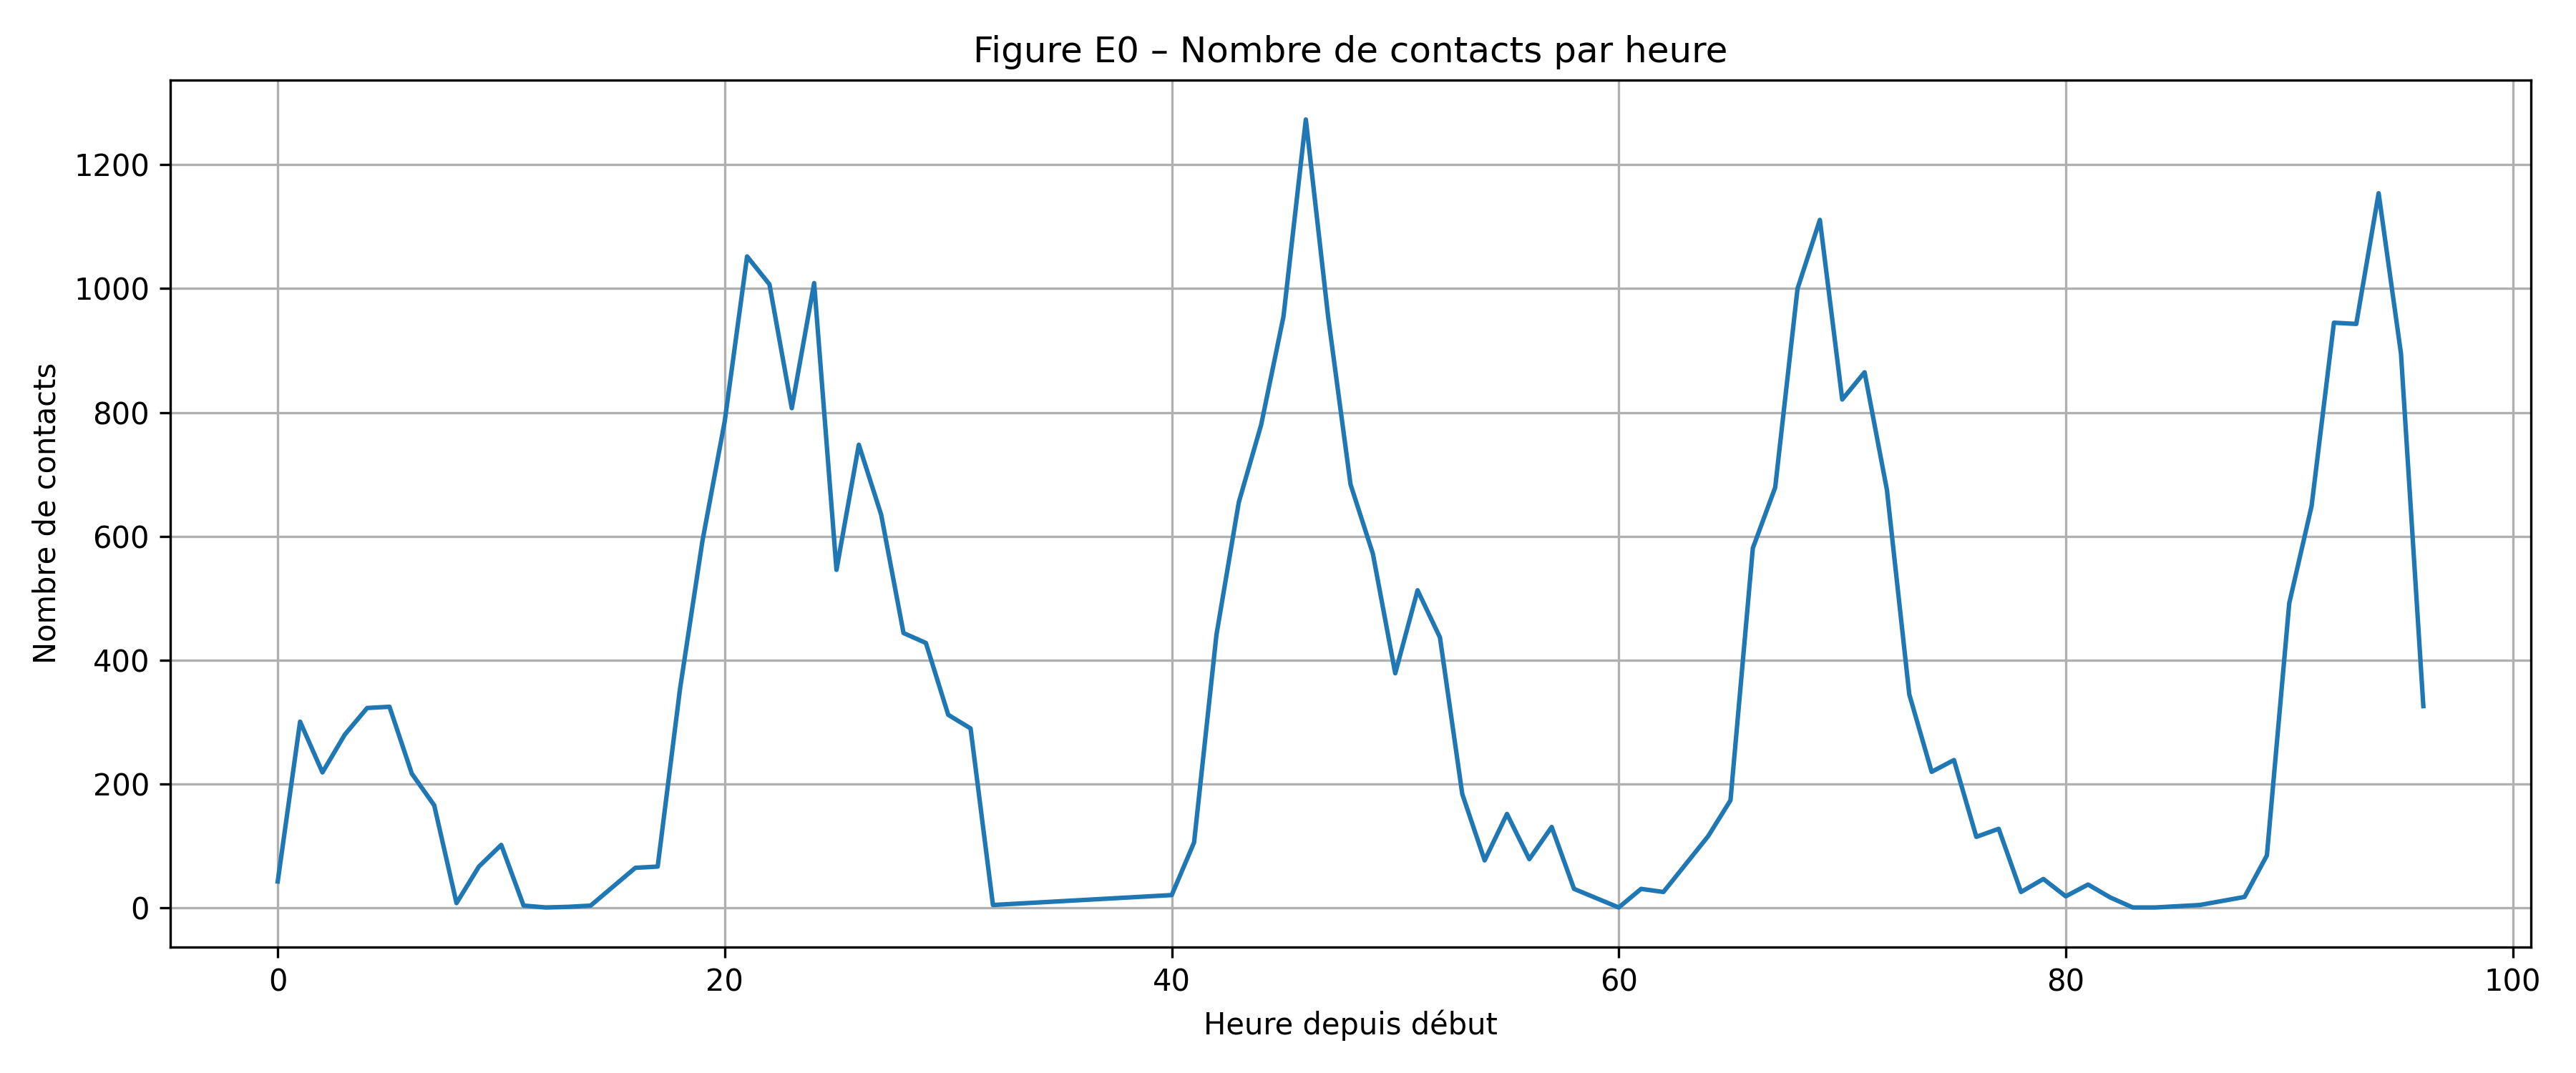
\includegraphics[width=0.90\linewidth]{images/article1/Figure_E0_contacts_par_heure.png}
\caption{Nombre total de contacts par heure.}
\end{figure}

Nous observons une structure \textbf{fortement cyclique}, caractérisée par :

\begin{itemize}
    \item des \textbf{pics très marqués} correspondant aux heures de service du personnel soignant ;
    \item des \textbf{creux importants} durant les périodes nocturnes ;
    \item des cycles réguliers, indicateurs d'une organisation journalière stable.
\end{itemize}

Ce phénomène est cohérent avec le schéma classique des \textbf{réseaux humains rythmiques}, typiques des organisations structurées comme les hôpitaux.

\subsection{Contacts par type d'interaction}

Pour comprendre la dynamique sociale interne, nous analysons les interactions par rôles.

\begin{figure}[H]
\centering
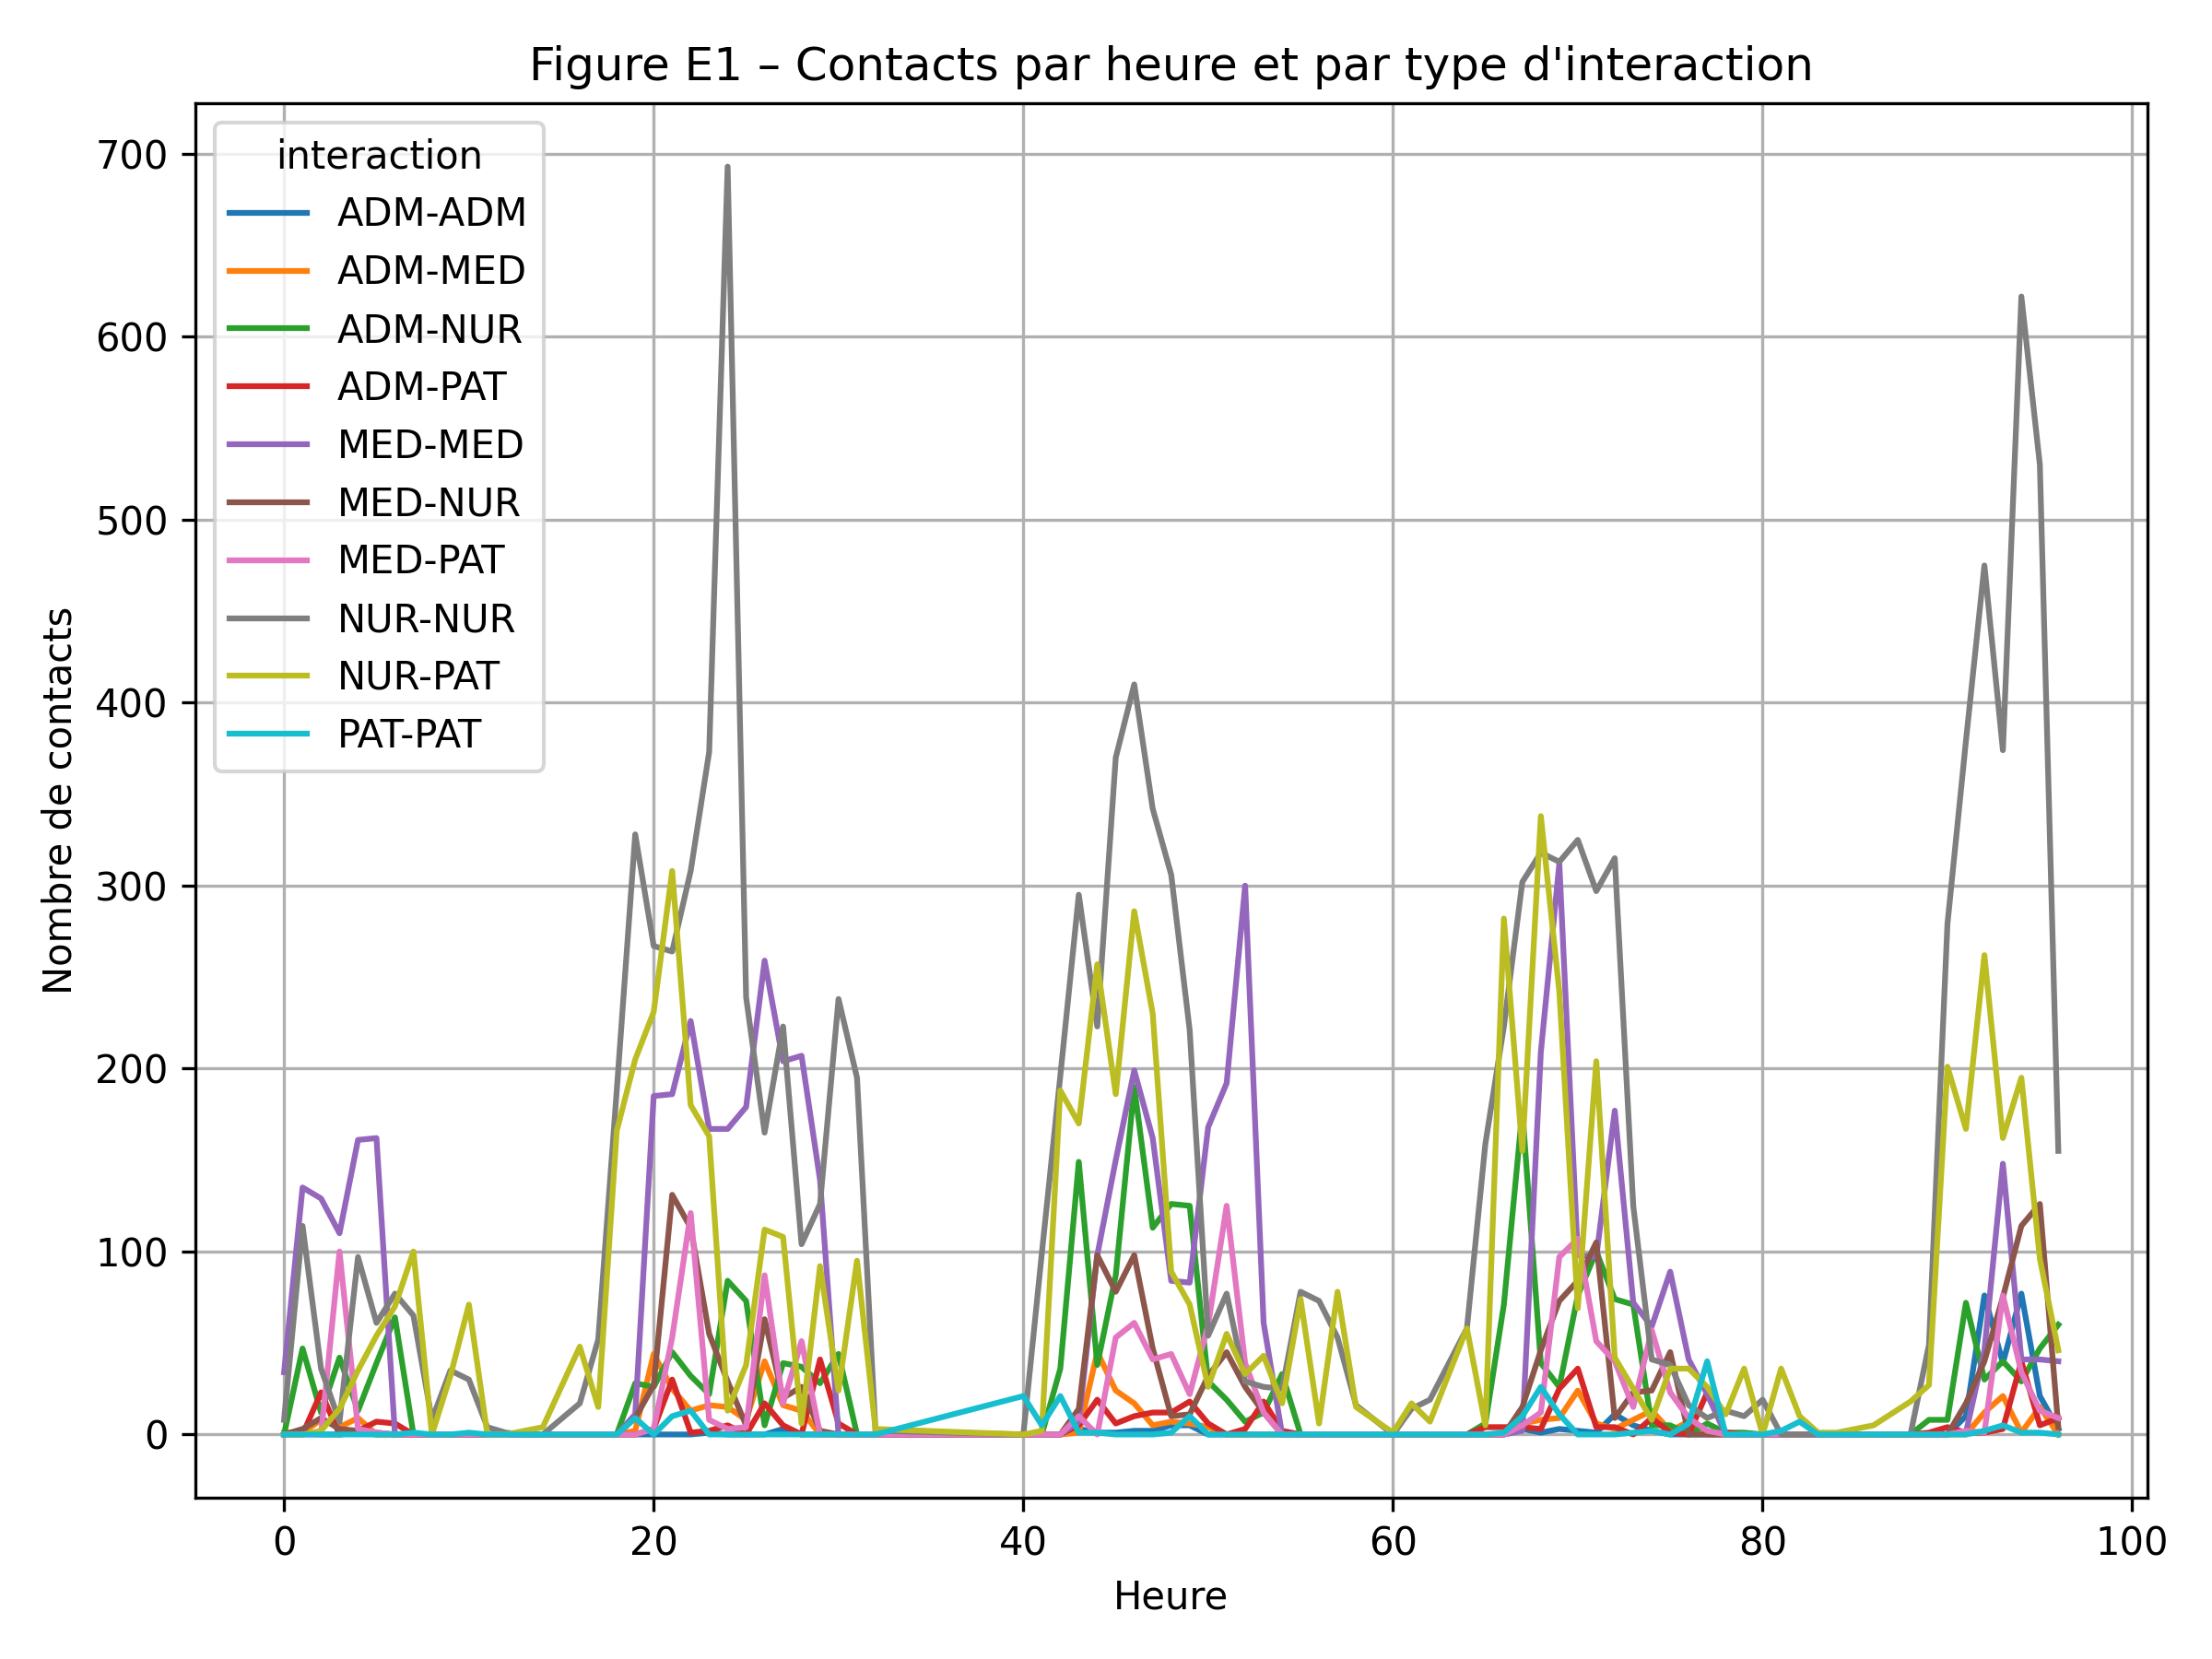
\includegraphics[width=0.90\linewidth]{images/article1/Figure_E1_contacts_par_role.png}
\caption{Contacts par heure selon le type d'interaction.}
\end{figure}

Les observations clés sont :

\begin{itemize}
    \item les contacts \textbf{NUR--PAT} et \textbf{NUR--NUR} dominent nettement, reflétant leur rôle opérationnel central ;
    \item les médecins interagissent surtout avec les infirmiers et peu directement avec les patients ;
    \item les contacts ADM restent faibles, souvent limités à leur propre catégorie.
\end{itemize}

Ces résultats montrent une \textbf{division fonctionnelle claire}. Les infirmiers constituent le point de contact principal entre les patients et l'organisation hospitalière.

% ============================================================
\section{Stabilité du voisinage : Similarité de Jaccard}
% ============================================================

\subsection{Concept théorique}

La similarité de Jaccard permet de quantifier la \textbf{stabilité} des contacts d'un individu entre deux jours successifs :

\[
J(i) = \frac{|N_1(i)\cap N_2(i)|}{|N_1(i)\cup N_2(i)|}.
\]

Un Jaccard élevé indique un voisinage stable ; une valeur faible signale des interactions changeantes.

\subsection{Résultats}

\begin{figure}[H]
\centering
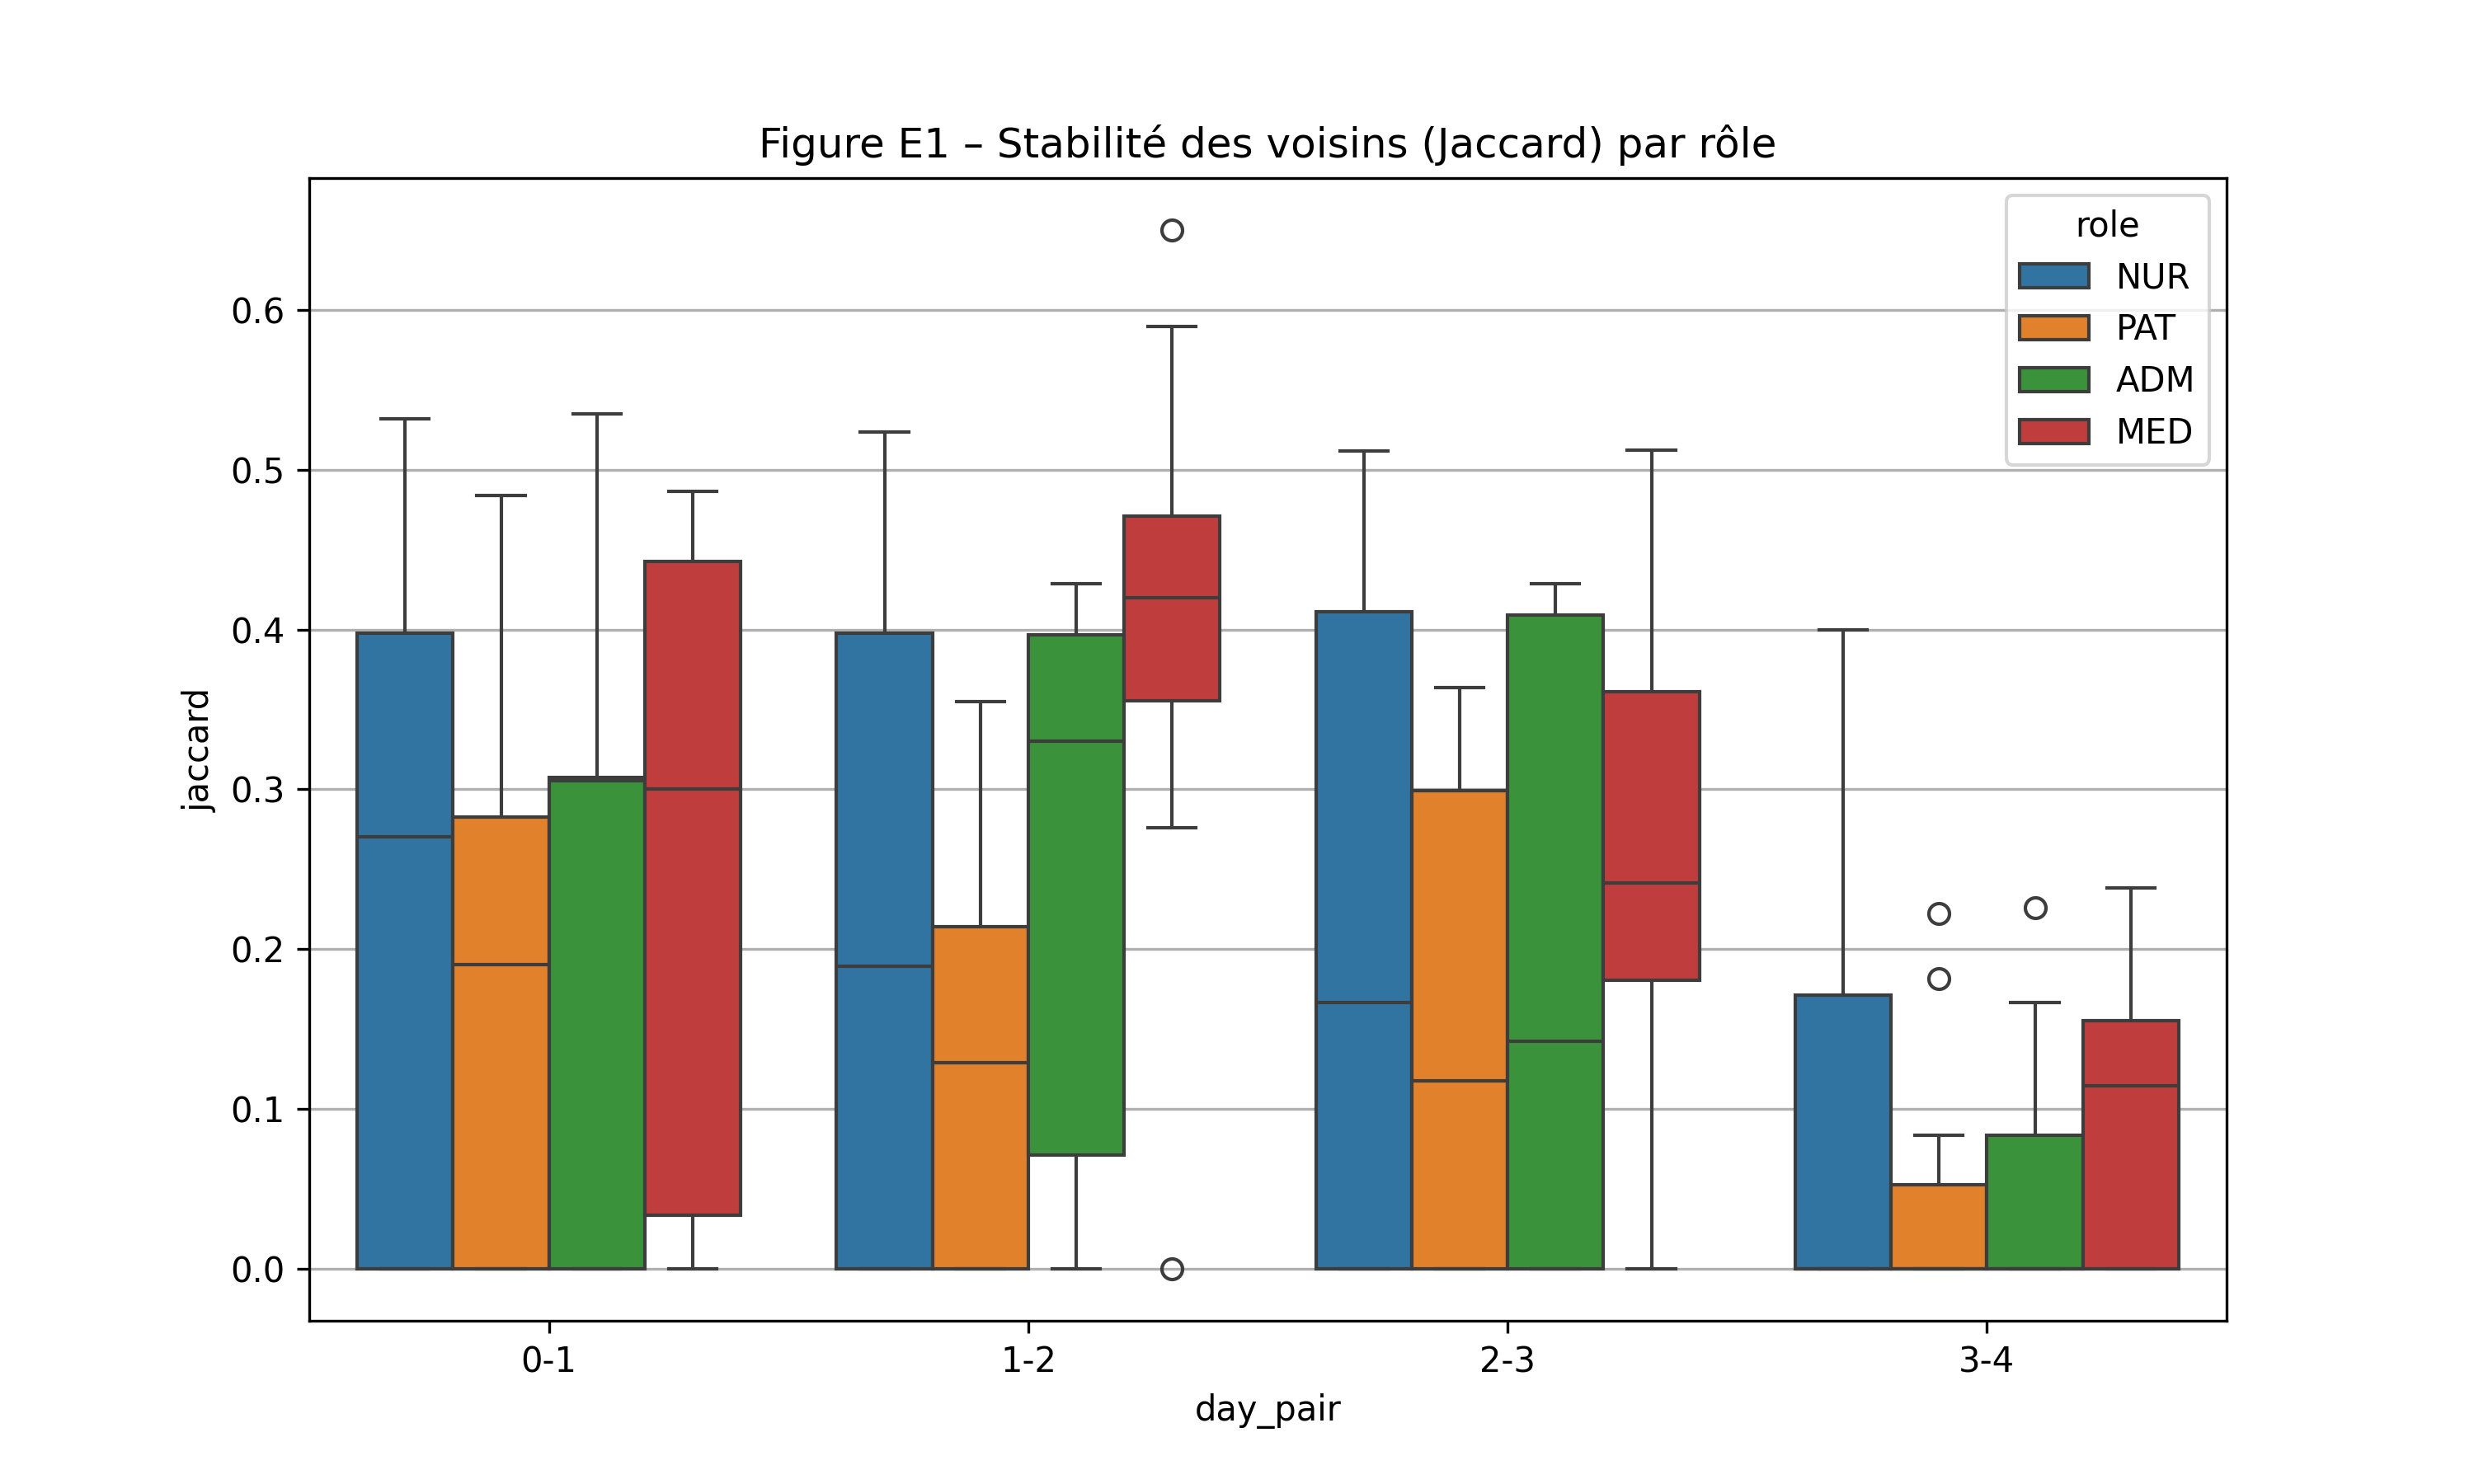
\includegraphics[width=0.85\linewidth]{images/article1/Figure_E1_stabilite_voisinage.png}
\caption{Stabilité des voisinages (Jaccard) par rôle.}
\end{figure}

Les résultats montrent :

\begin{itemize}
    \item une \textbf{forte stabilité} pour les infirmiers (NUR), cohérente avec des équipes fixes ;
    \item une stabilité moyenne pour les médecins (MED) ;
    \item une \textbf{faible stabilité} pour les patients (PAT), dont les interactions dépendent de leur état, des soins dispensés et des déplacements.
\end{itemize}

Cette analyse démontre que la \textbf{structure sociale interne est stable pour le personnel mais dynamique pour les patients}.

% ============================================================
\section{Structure temporelle du réseau}
% ============================================================

\subsection{Diamètre}

Le diamètre d'un graphe reflète l'étendue maximale des plus courts chemins.

\begin{figure}[H]
\centering
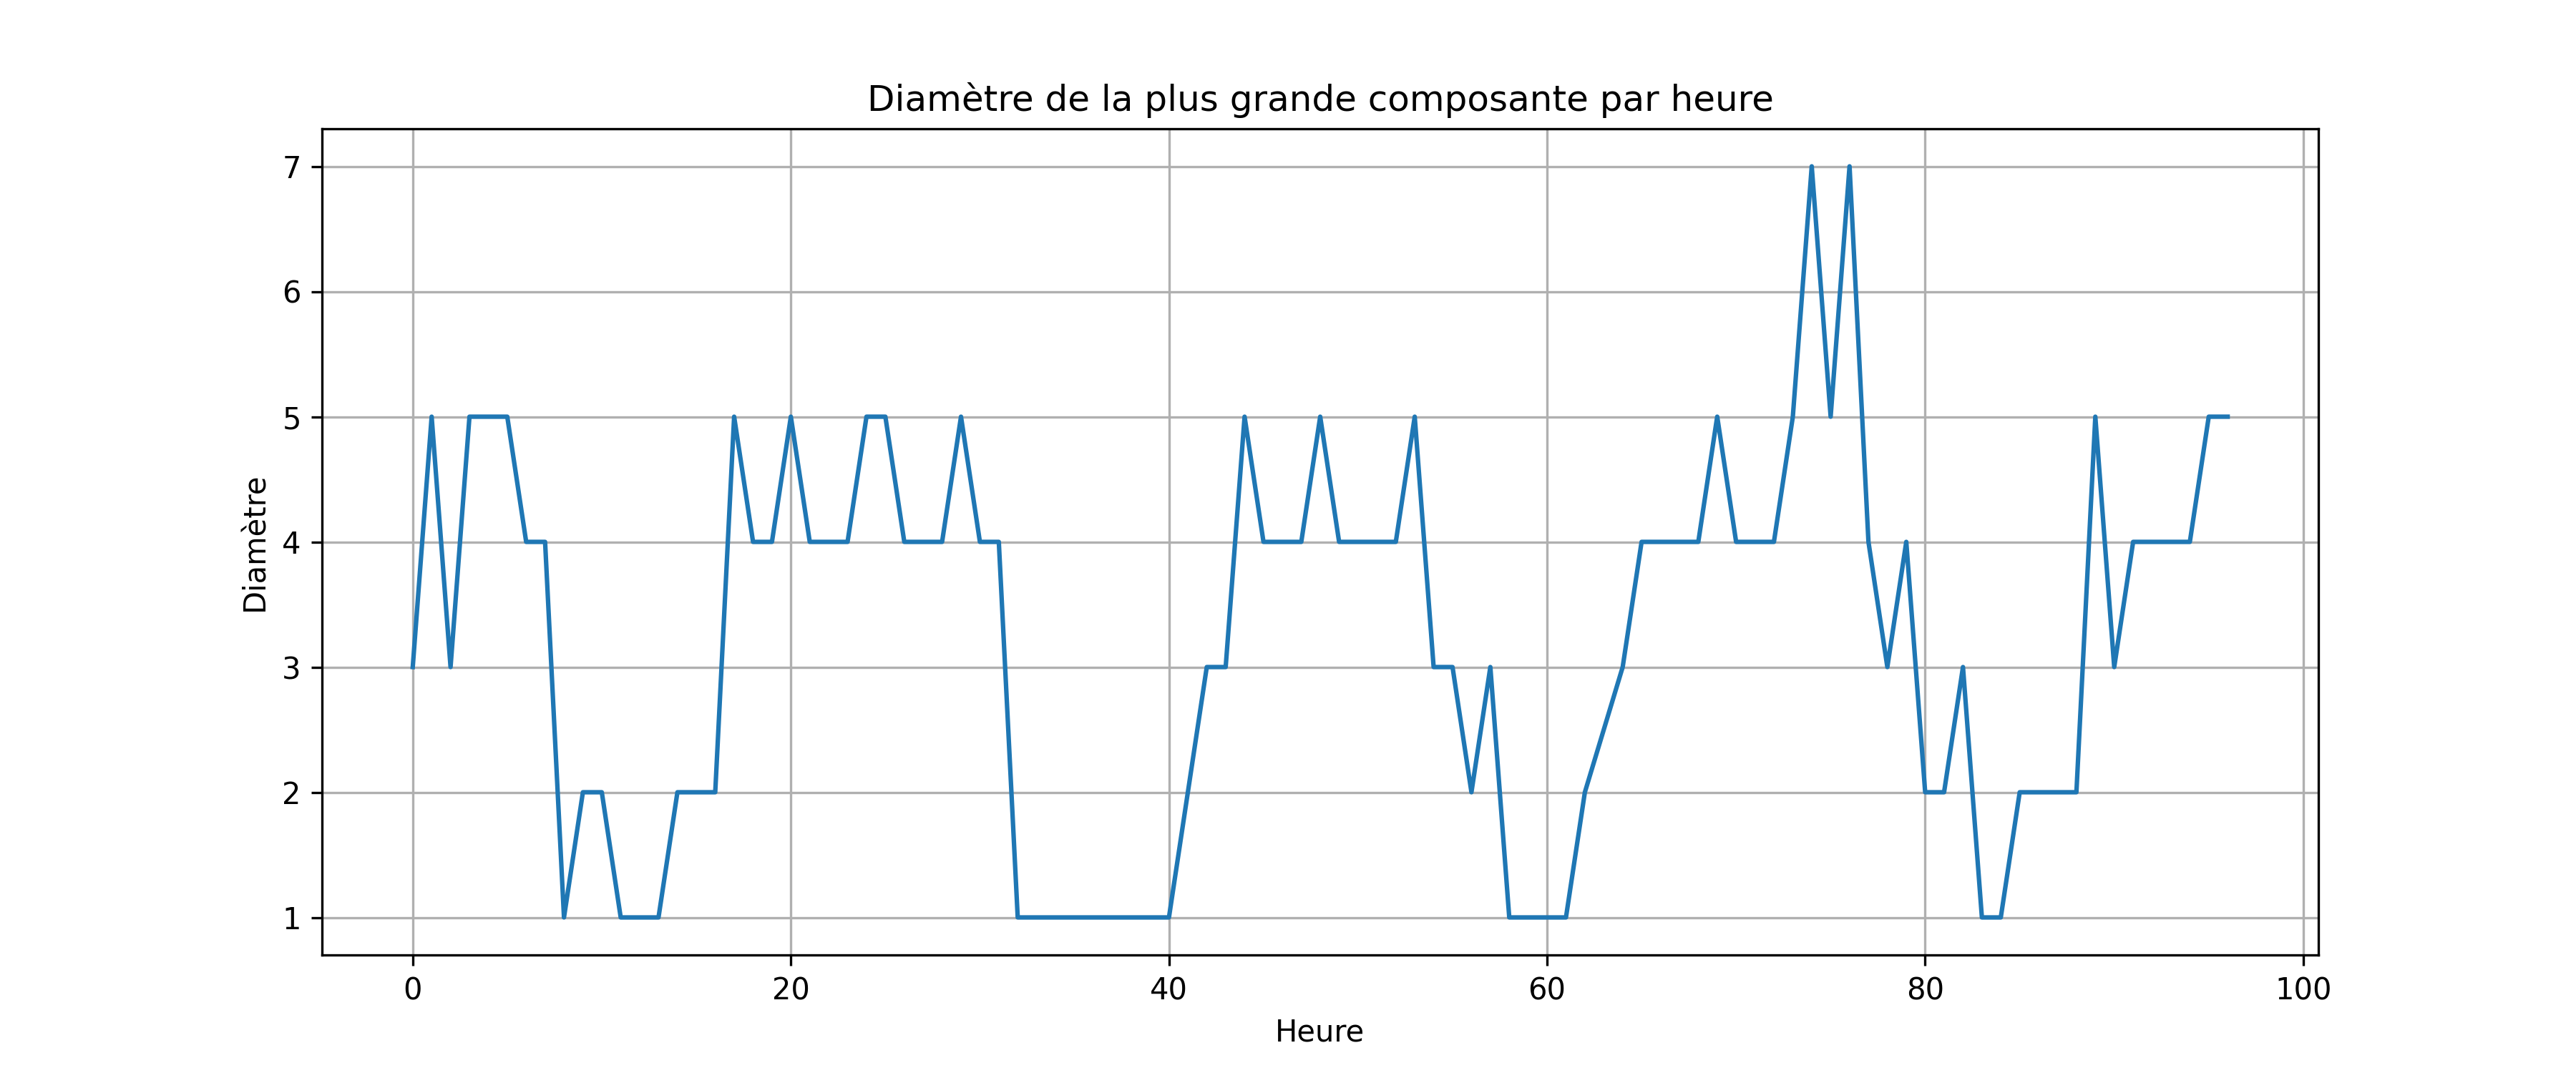
\includegraphics[width=0.90\linewidth]{images/article1/Figure_E2_diametre.png}
\caption{Diamètre de la plus grande composante.}
\end{figure}

Nous constatons un diamètre compris entre 3 et 7, indiquant un réseau :

\begin{itemize}
    \item \textbf{compact}, où la distance maximale reste faible ;
    \item robuste à la fragmentation ;
    \item proche d'une structure \textbf{small-world}.
\end{itemize}

\subsection{Distance moyenne}

\begin{figure}[H]
\centering
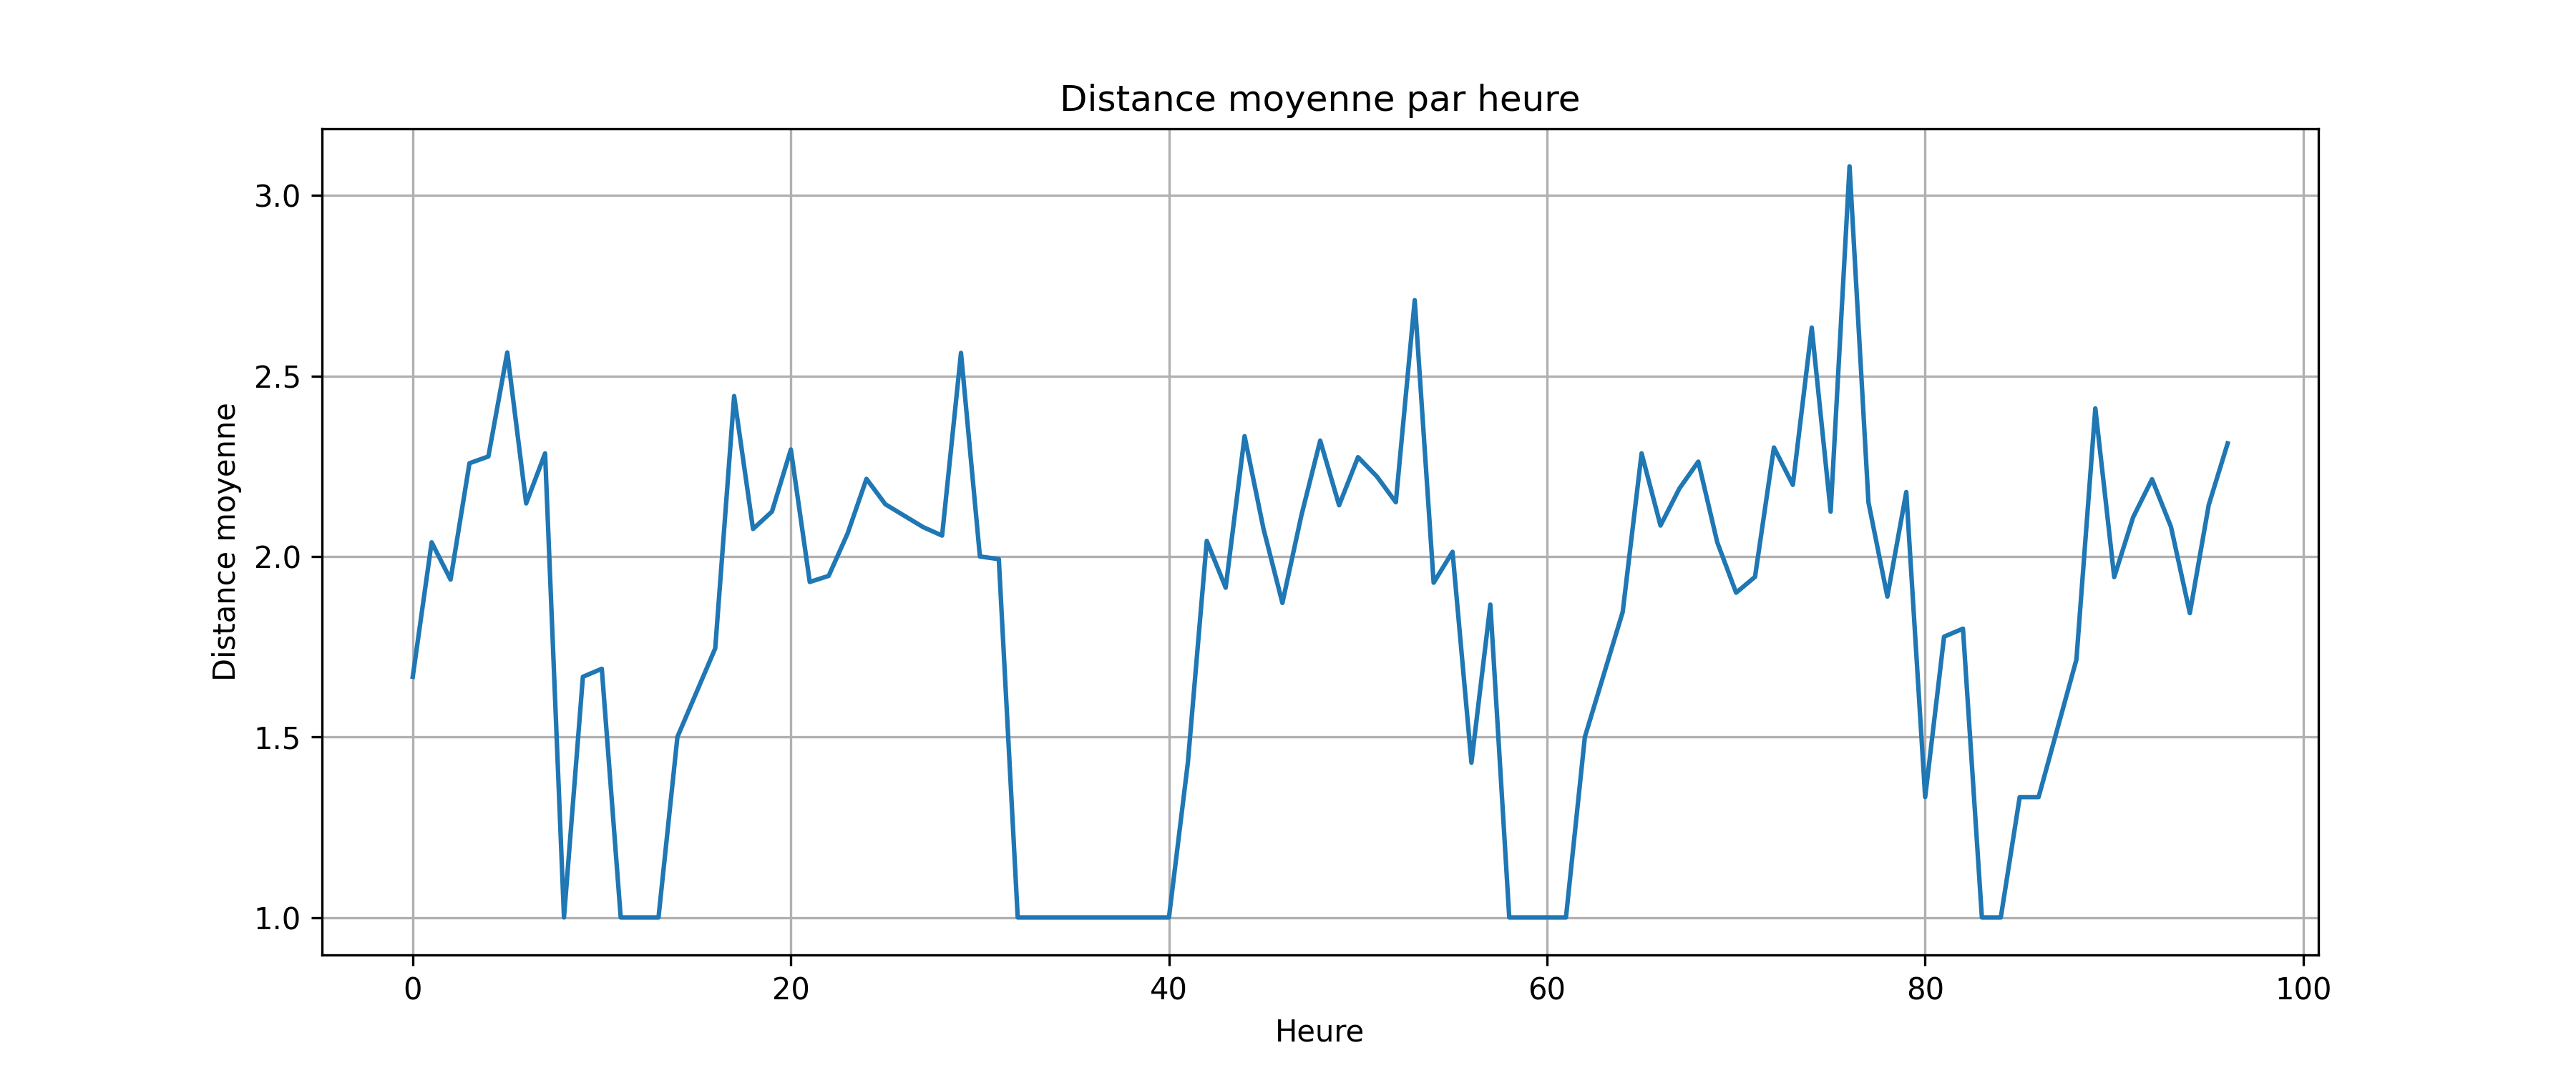
\includegraphics[width=0.90\linewidth]{images/article1/Figure_E3_distance_moyenne.png}
\caption{Distance moyenne par heure.}
\end{figure}

La distance moyenne (1.8 à 2.6) confirme la compacité du réseau :

\begin{itemize}
    \item propagation rapide de l'information ;
    \item interactions fortement interconnectées ;
    \item absence de barrières structurelles fortes.
\end{itemize}

\subsection{Nombre de composantes}

\begin{figure}[H]
\centering
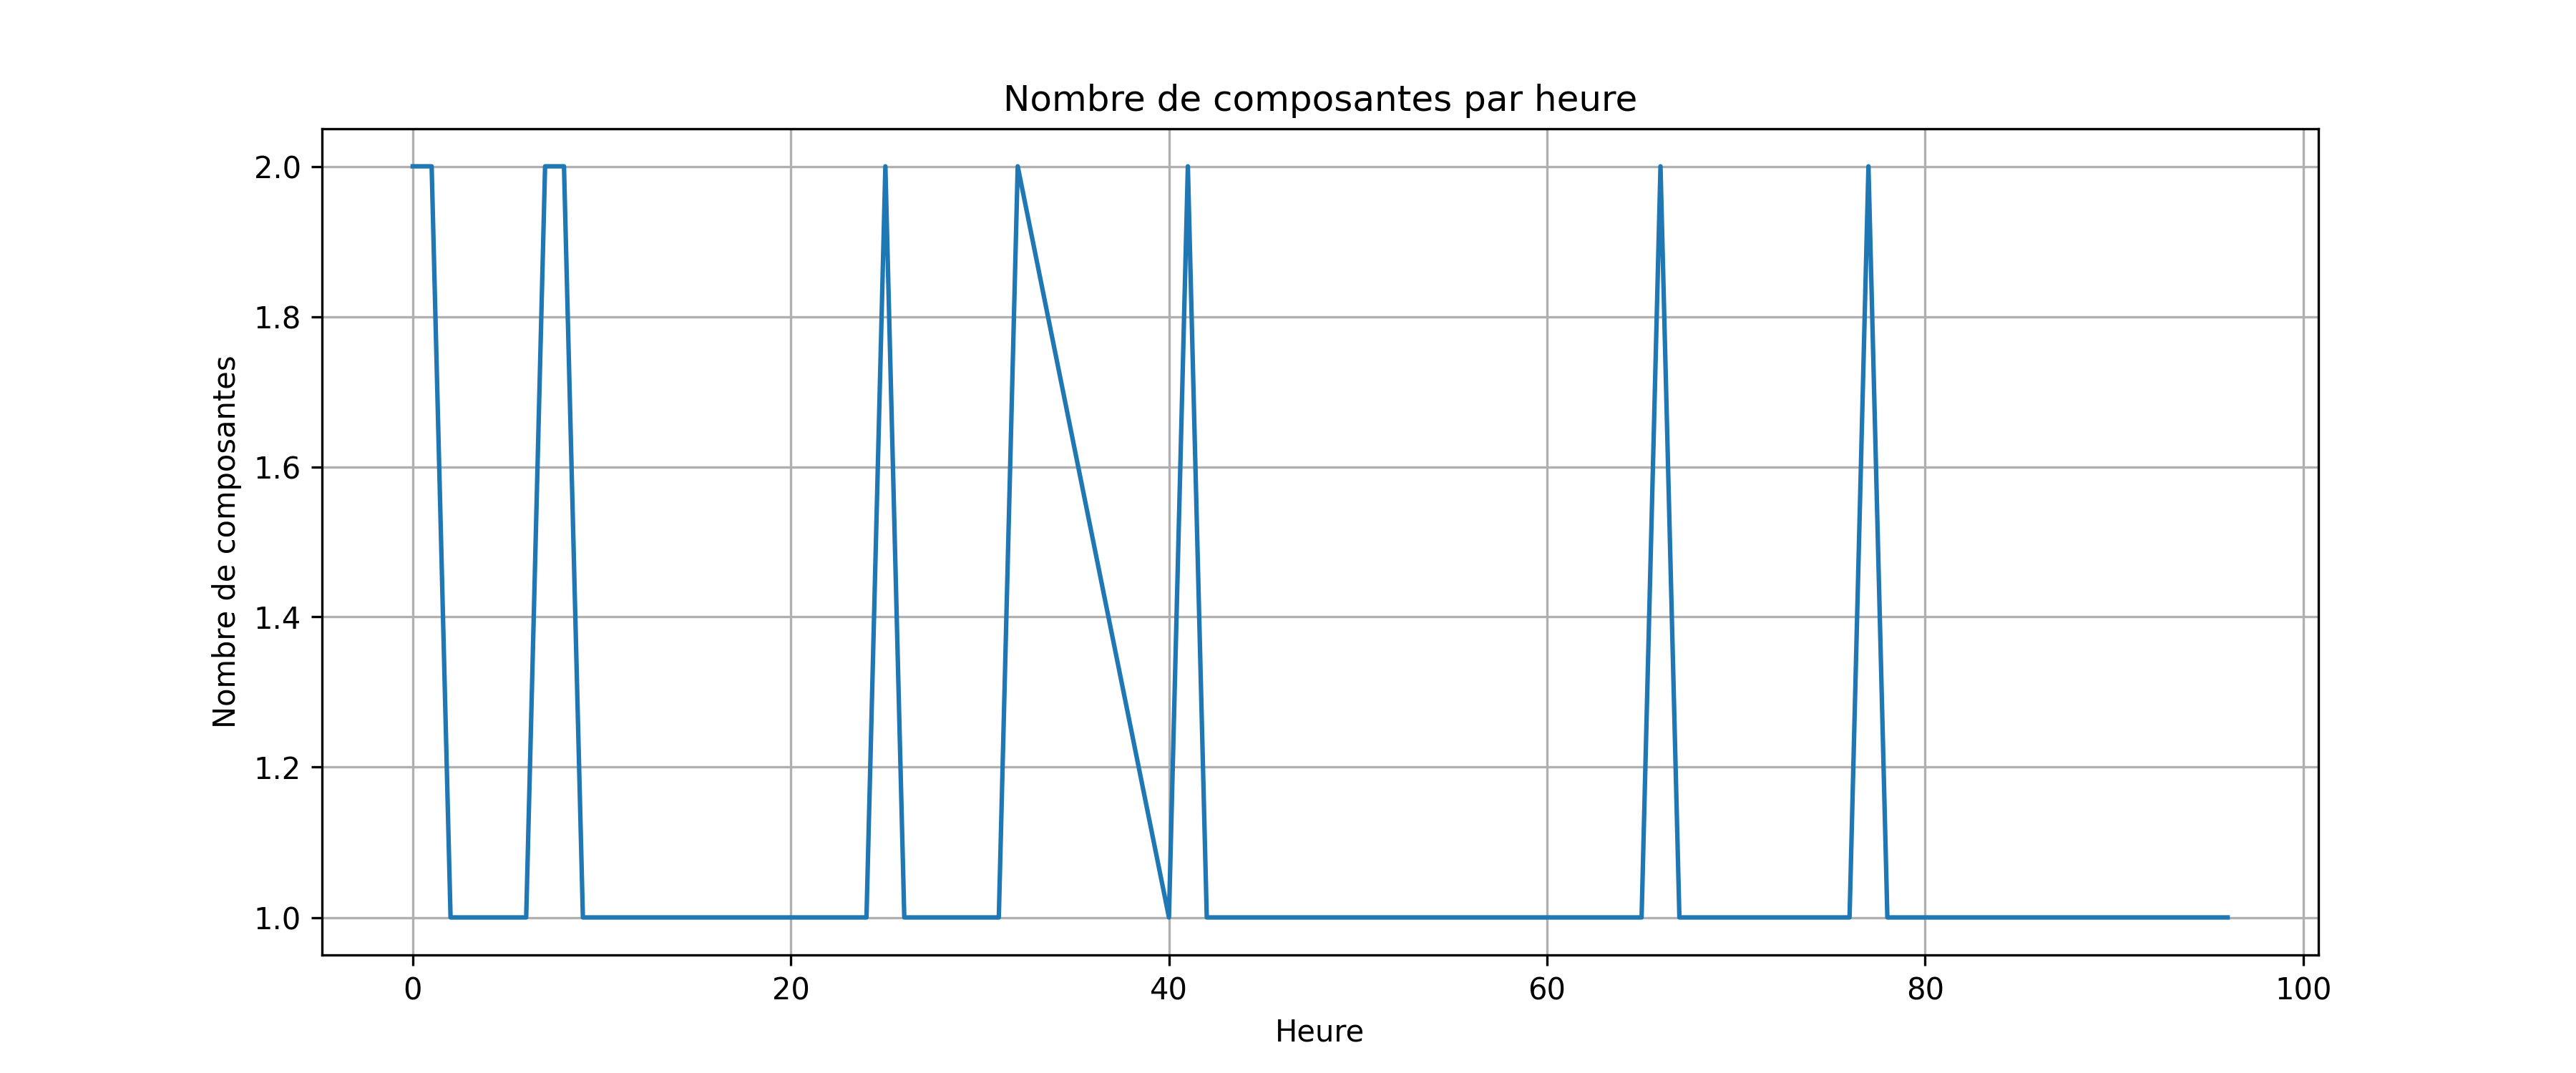
\includegraphics[width=0.90\linewidth]{images/article1/Figure_E4_composantes.png}
\caption{Nombre de composantes du graphe.}
\end{figure}

Le réseau reste connecté la quasi-totalité du temps, ce qui indique une \textbf{forte cohésion structurelle}.

% ============================================================
\section{Analyse du graphe agrégé}
% ============================================================

\subsection{Visualisation brute}

\begin{figure}[H]
\centering
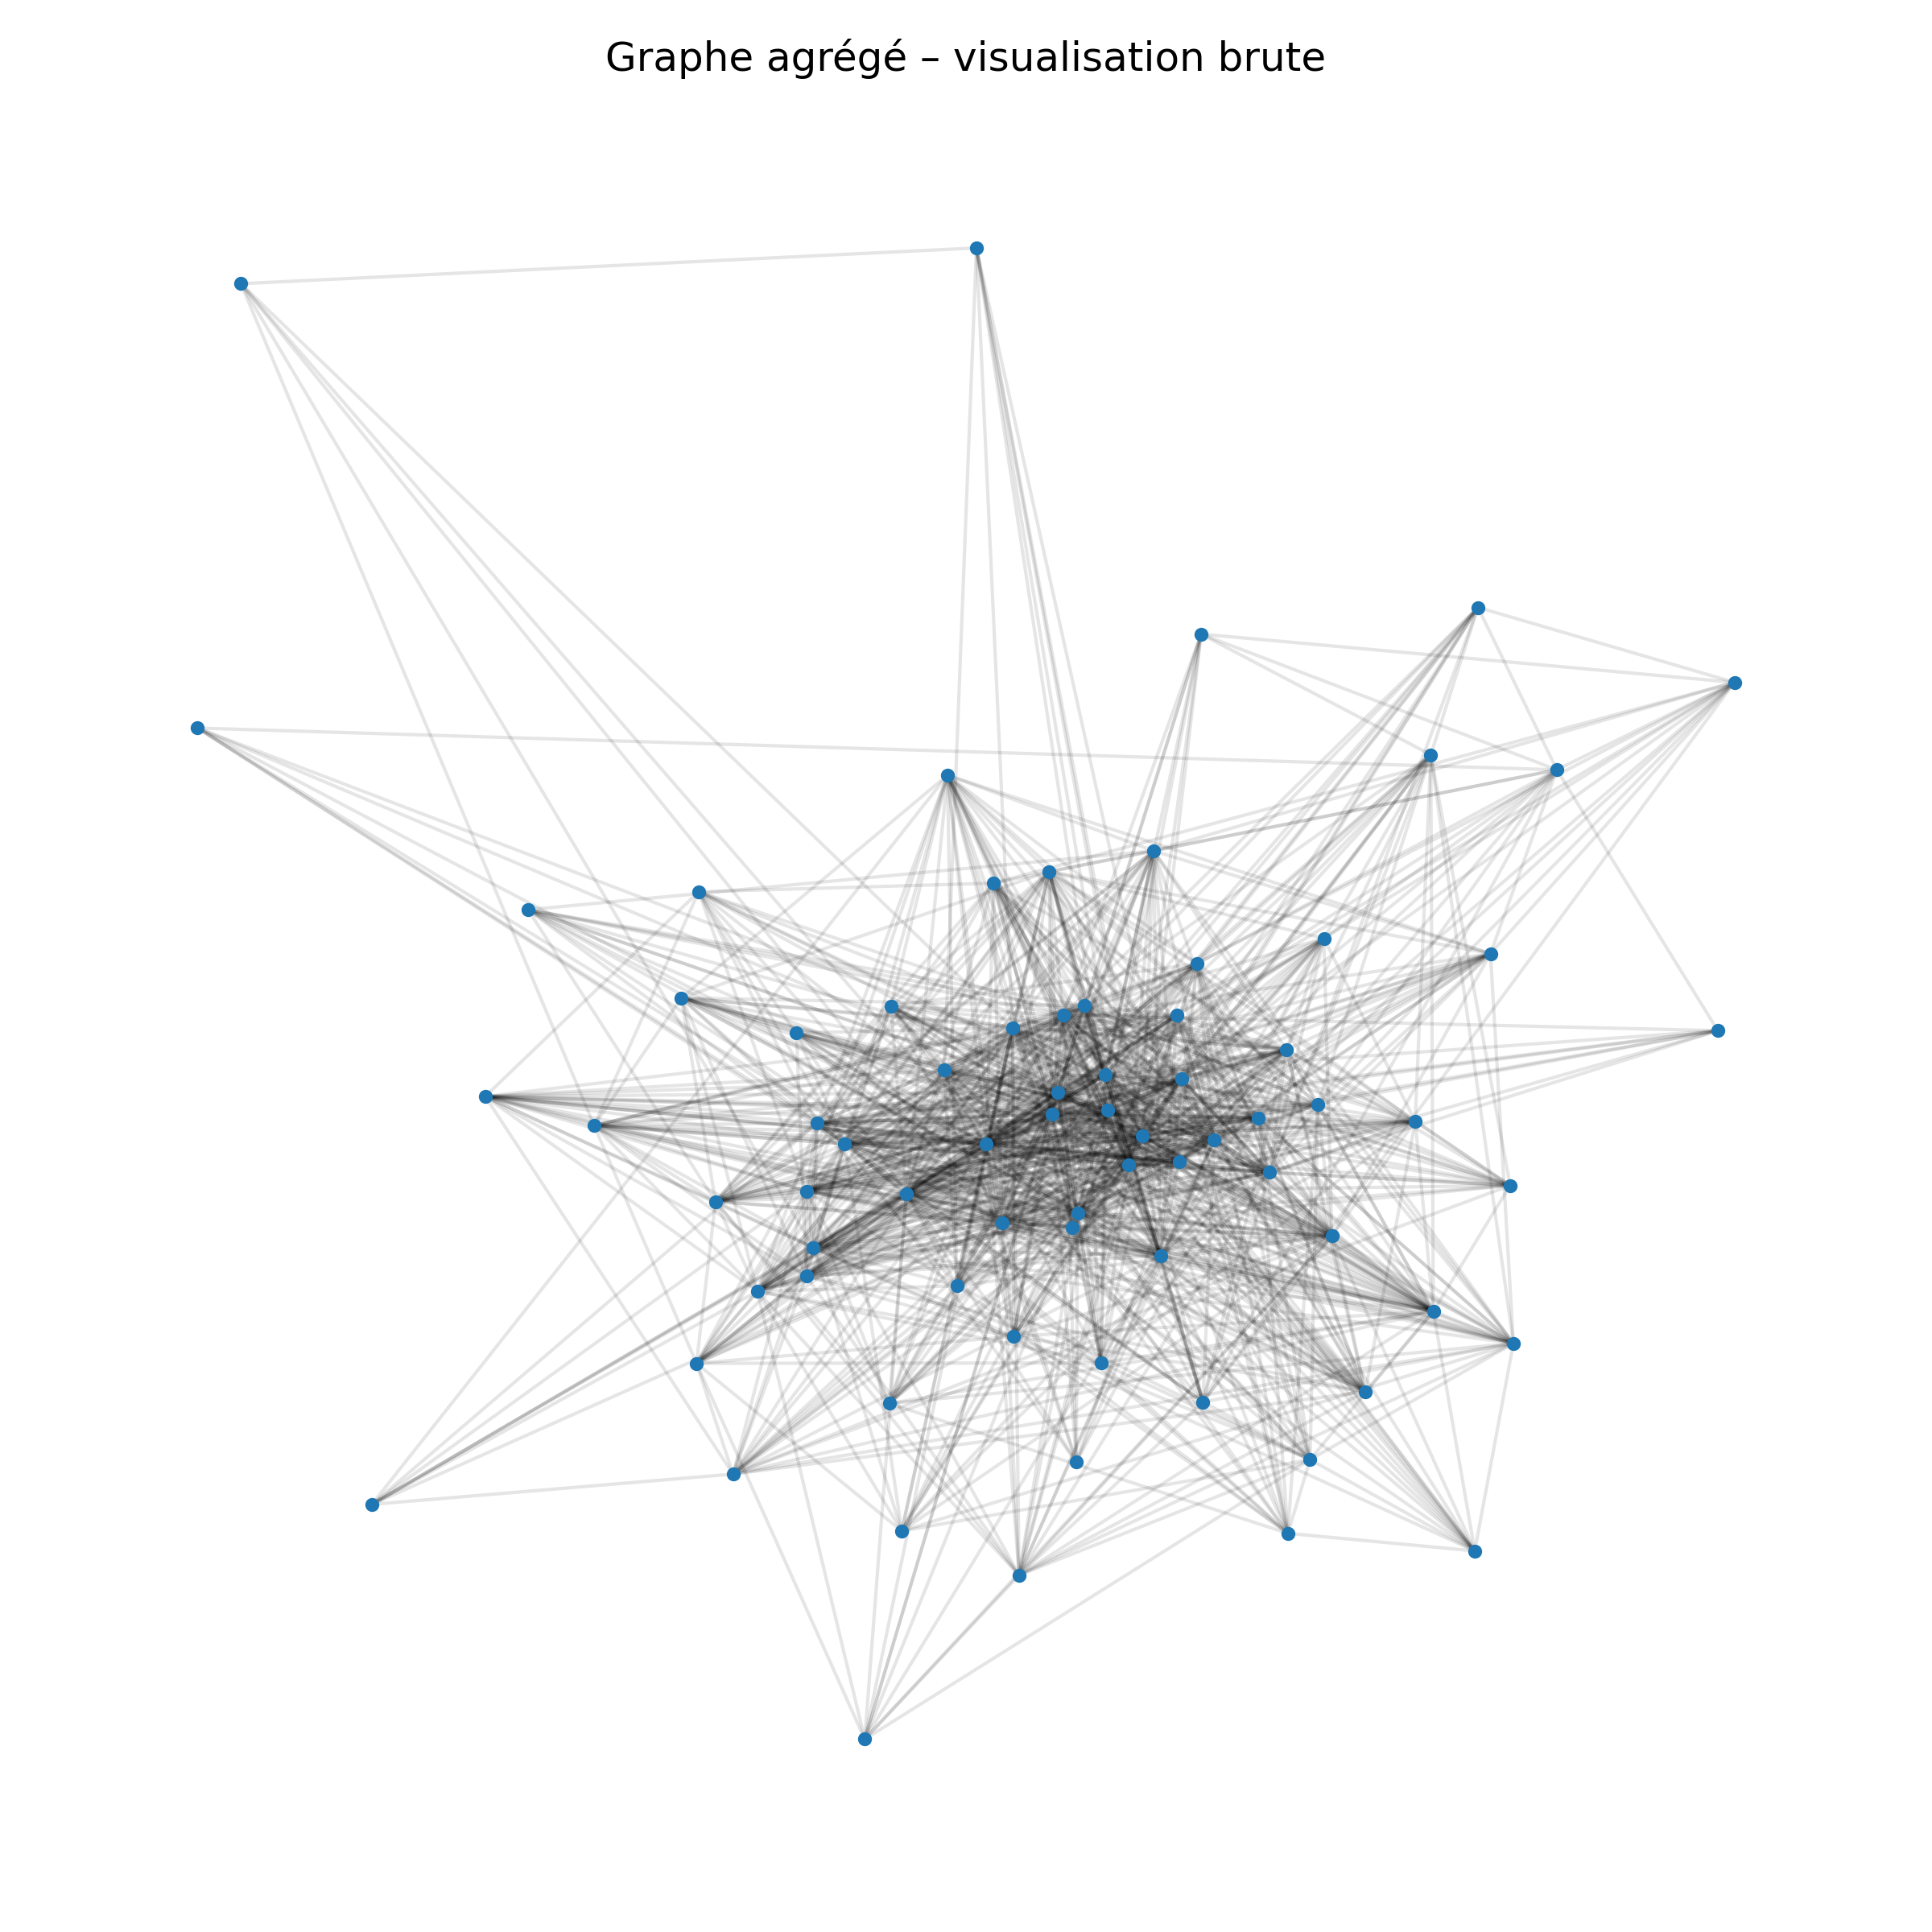
\includegraphics[width=0.75\linewidth]{images/Figure_D0_graphe_brut.png}
\caption{Graphe agrégé : visualisation brute.}
\end{figure}

Le graphe est dense : 75 nœuds, 1139 arêtes. La zone centrale apparaît saturée, illustrant une forte activité interne du personnel.

\subsection{Communautés (Louvain)}

\begin{figure}[H]
\centering
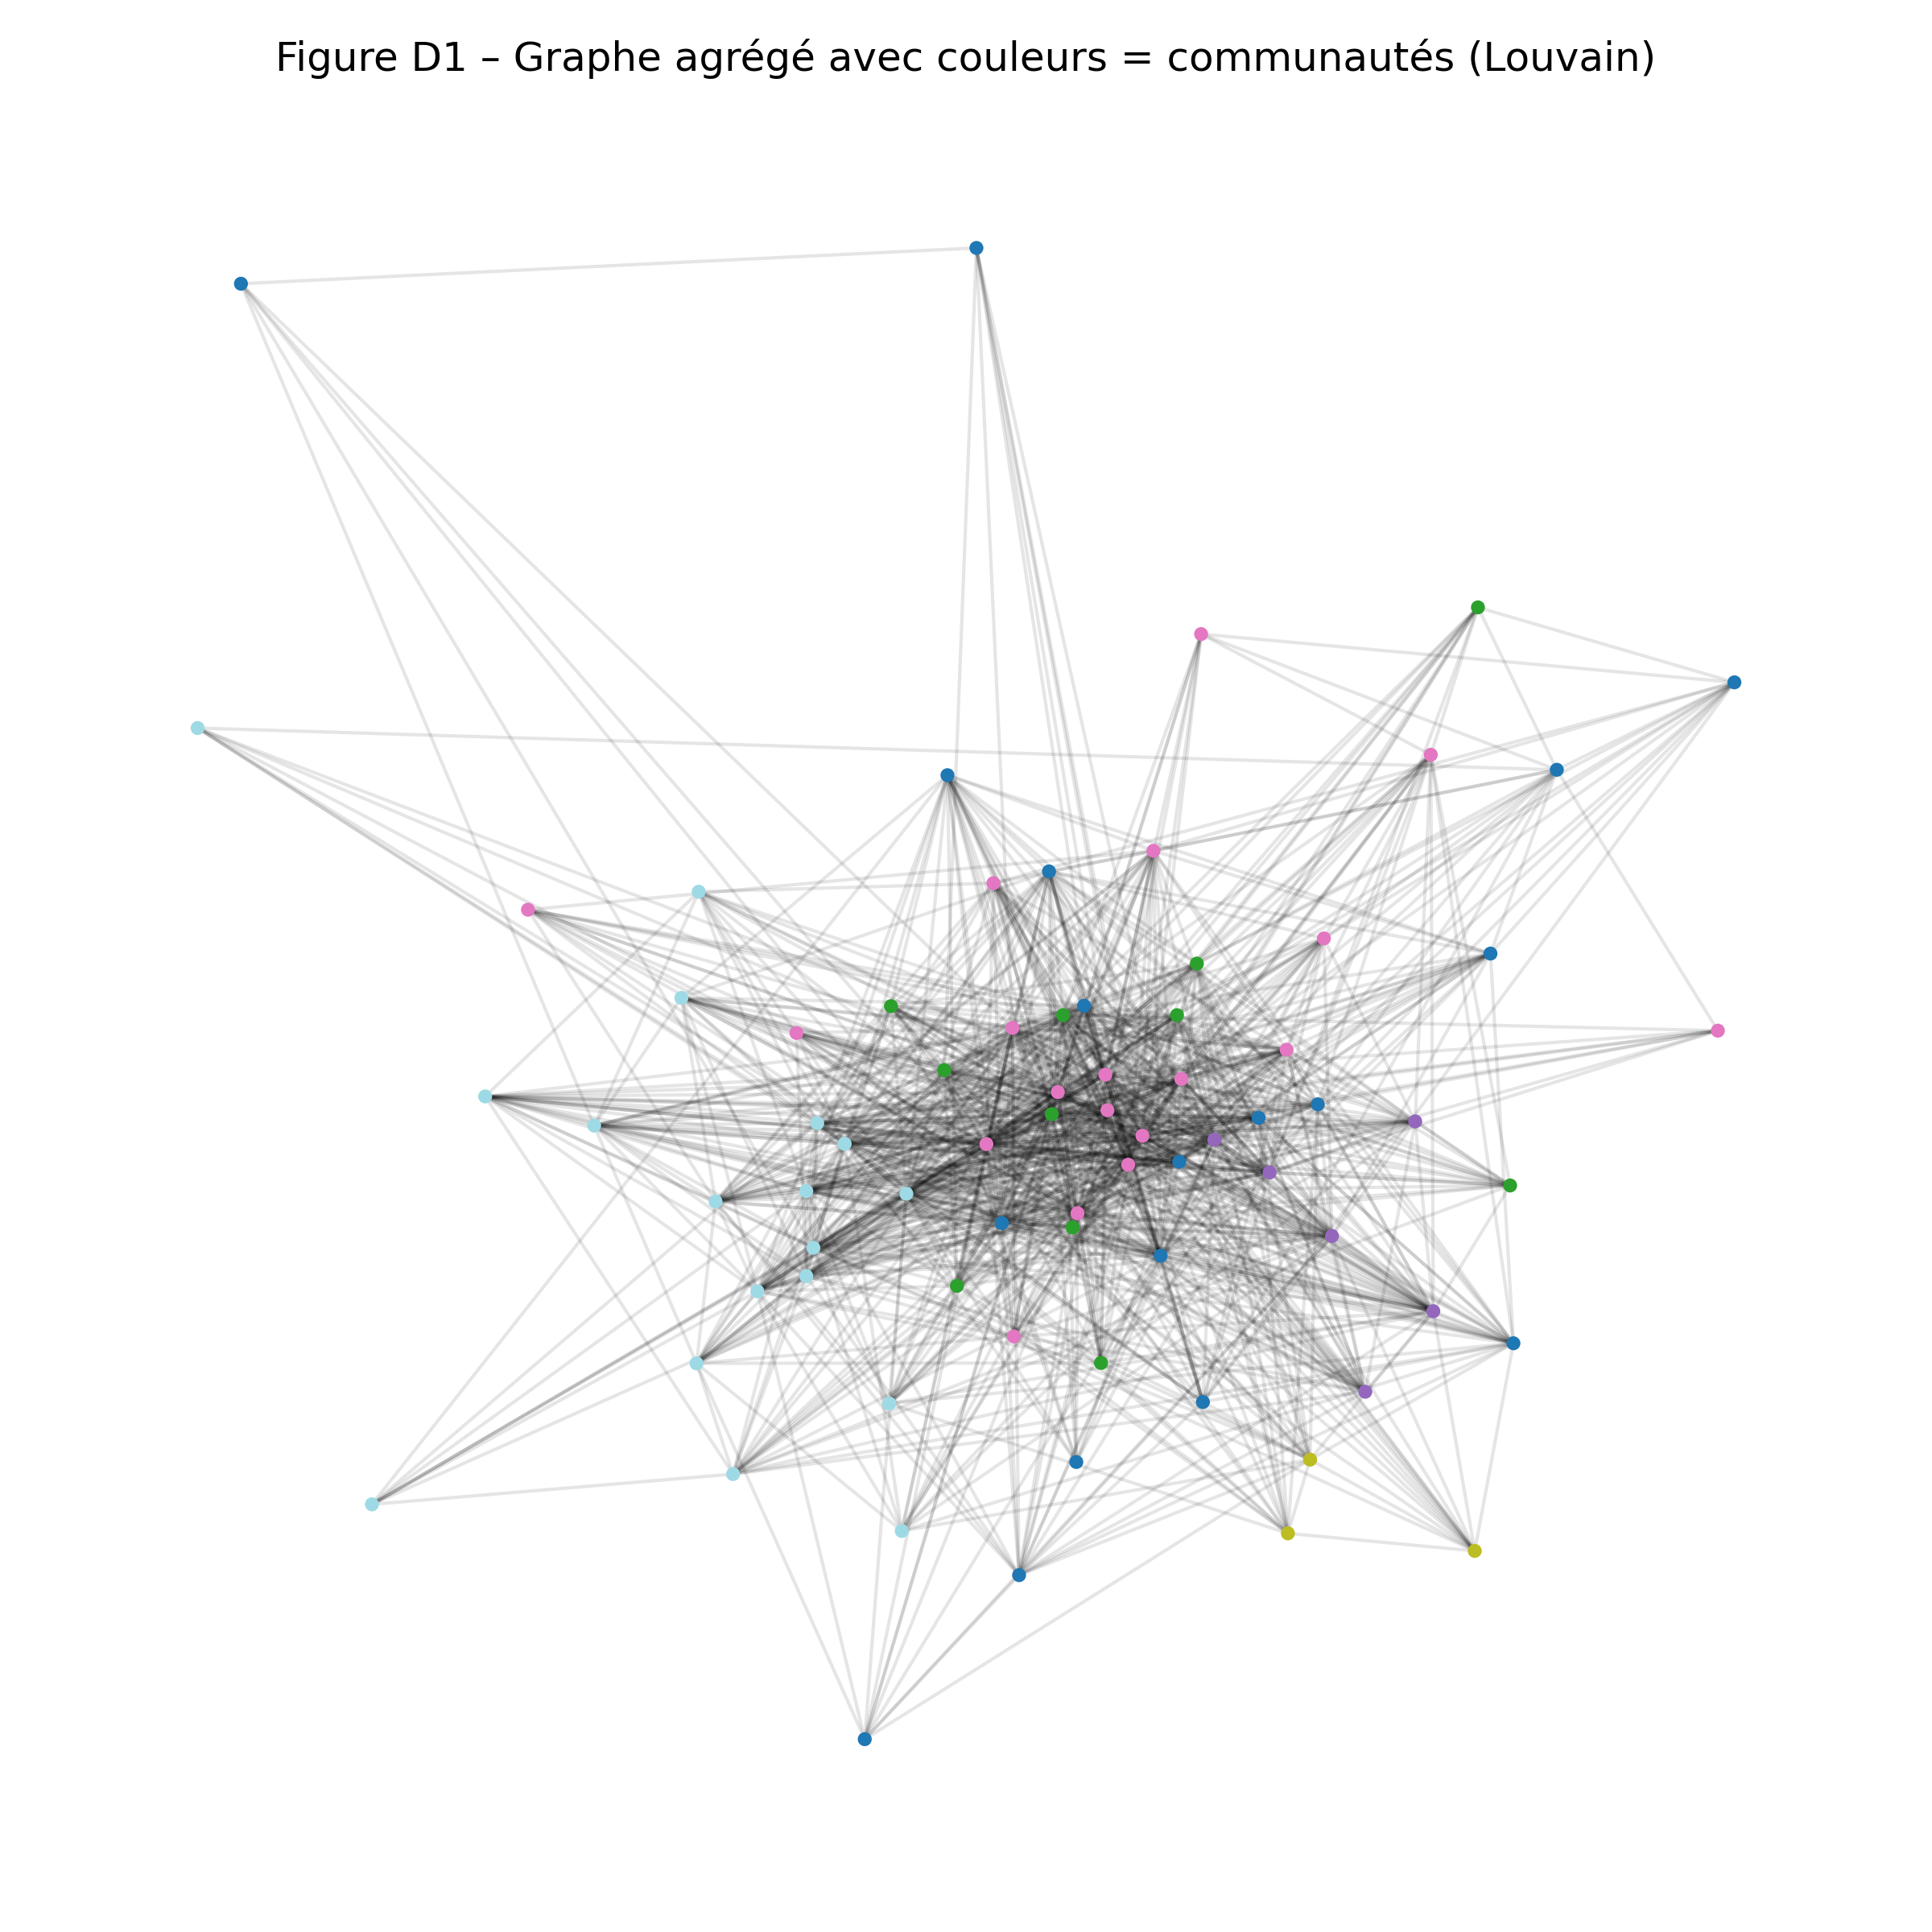
\includegraphics[width=0.75\linewidth]{images/article1/Figure_D1_communautes_Louvain.png}
\caption{Communautés détectées (Louvain).}
\end{figure}

\begin{figure}[H]
\centering
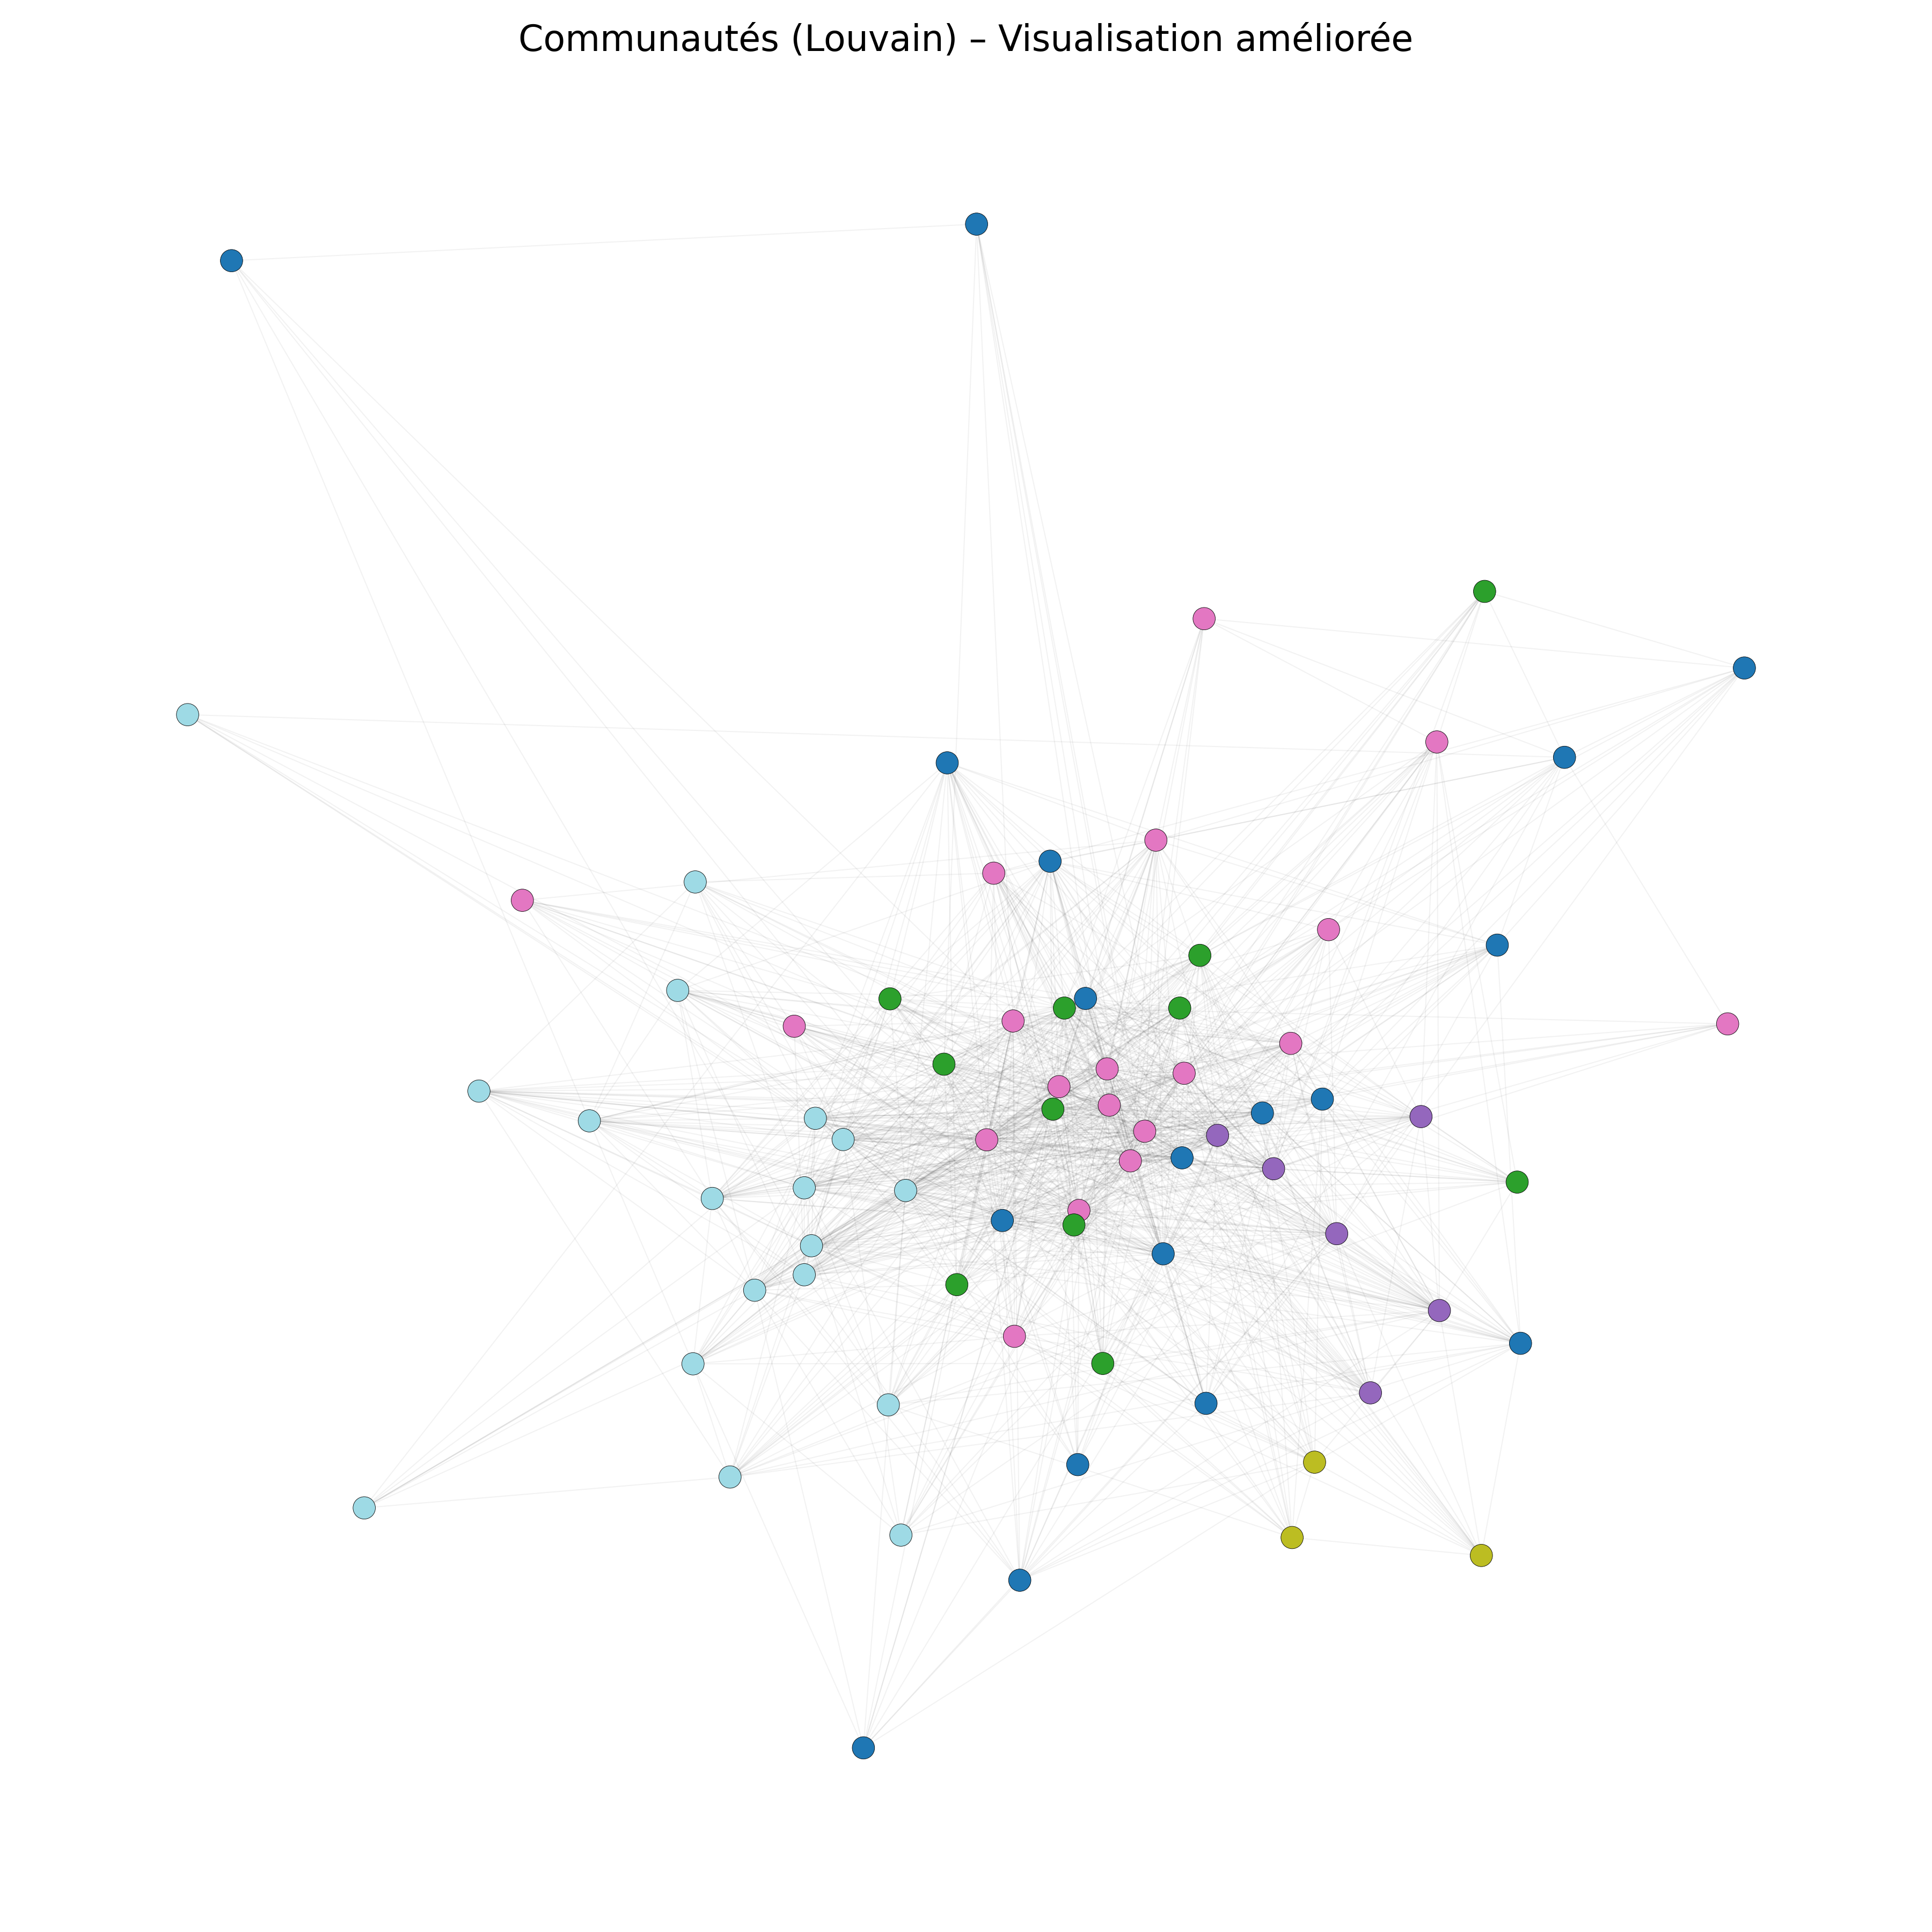
\includegraphics[width=0.75\linewidth]{images/article1/Figure_D1_communautes_améliorée.png}
\caption{Visualisation améliorée.}
\end{figure}

La modularité de 0.368 révèle une \textbf{structure communautaire modérée}. Les communautés correspondent probablement à :

\begin{itemize}
    \item différents groupes de soignants ;
    \item équipes opérationnelles ;
    \item clusters patients–infirmiers.
\end{itemize}

% ============================================================
\section{Analyse core--périphérie (k-core)}
% ============================================================

\begin{figure}[H]
\centering
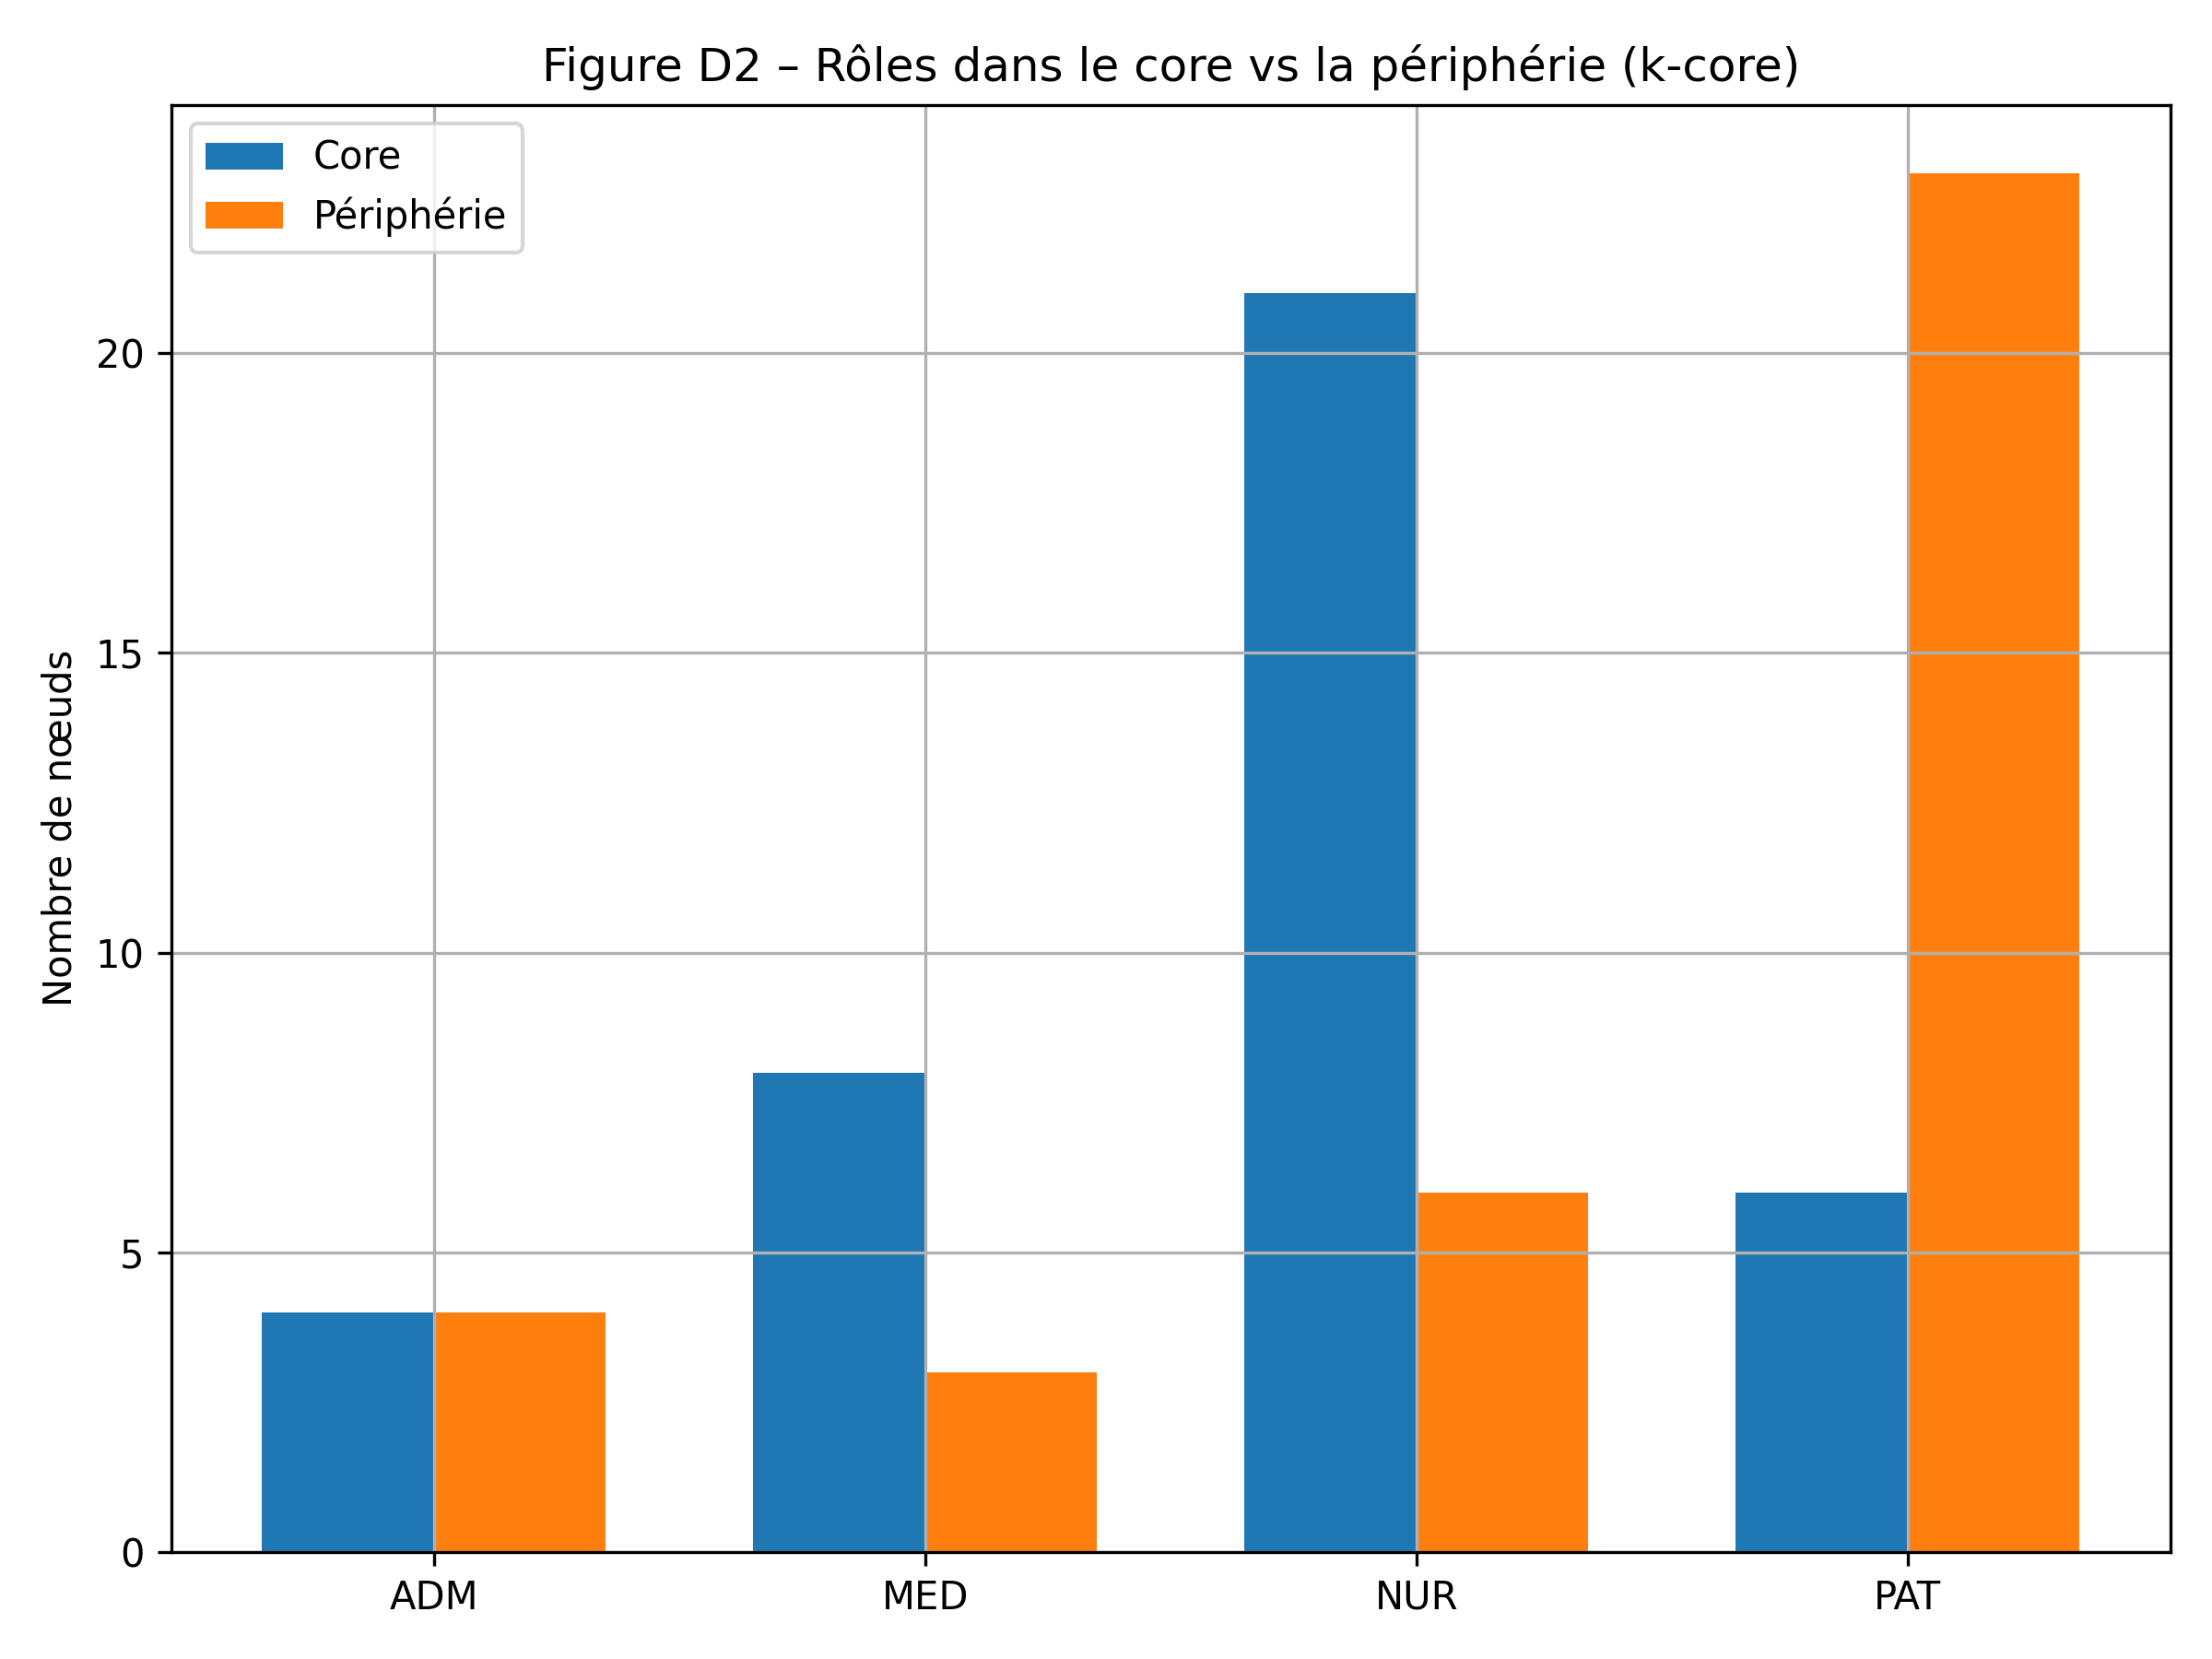
\includegraphics[width=0.85\linewidth]{images/article1/Figure_D2_core_vs_periphery_roles.png}
\caption{Répartition des rôles dans le core et la périphérie.}
\end{figure}

Le $k$-core maximal est 22 : très élevé pour un réseau de 75 nœuds.

Le \textbf{core} est dominé par :

\begin{itemize}
    \item 21 NUR ;
    \item 8 MED ;
    \item quelques ADM et PAT.
\end{itemize}

La \textbf{périphérie} contient surtout des patients (23).

Cela indique que le réseau est organisé autour d'un \textbf{noyau central fortement connecté}, principalement constitué d'infirmiers, pivot de la dynamique hospitalière.

% ============================================================
\section{Conclusion}
% ============================================================

L'analyse révèle :

\begin{itemize}
    \item une dynamique temporelle cyclique ;
    \item un rôle central des infirmiers dans la structure du réseau ;
    \item un réseau compact et fortement connecté ;
    \item une stabilité élevée du personnel mais variabilité des patients ;
    \item une organisation communautaire réelle ;
    \item une structure core--périphérie nette.
\end{itemize}

Ce réseau hospitalier apparaît comme un système dense, structuré par les rôles et rythmes opérationnels, avec un noyau central essentiel à son fonctionnement.

\end{document}